\documentclass[../main.tex]{subfiles}
\begin{document}

\thispagestyle{myheadings}


This chapter describes several projects that were started early during my graduate studies.
Each project is similar in that they are outside the realm of optical imaging of neural activity, which is the focus of the rest of this dissertation.
Nevertheless, they are included here because the issues they bring up will later inform the approach I take in the work described in later chapters.
The projects described in the following sections are also tied together by a common goal: to enable research in the neurosciences with translation potential for clinical applications.

\section{
  Animal Tracking}\label{animal-tracking}

\subsection{PD mouse model:}\label{pd-mouse-model}

You can induce a quantifiable PD-like state in mice with a unilateral injection of the neurotoxin 6-hydroxydopamine (6-OHDA) into the striatum, and subsequent administration of apomorphine to provoke side-biased motor deficits {[}@iancu\_behavioral\_2005{]}.
Side-biased``turning'' behavior is quantified autonomously on two distinct platforms, a computer-vision system that allows free movement, and a virtual-reality spherical treadmill platform that simulates free movement.

\subsection{
	Metrics of Behavior}\label{metrics-of-behavior}

Two testing platforms are used to assess changes in behavior over time.
Behavior is analyzed and quantified in real-time, and are synchronized with electrophysiology and made available as stream of events synchronized with imaging and/or electrophysiology.
The quantification routine creates a signal that is representative of symptom severity.
For our unilaterally lesioned mouse model of PD the most readily observable impairment is the inability to walk straight;
mice would turn in circles
contralateral to the lesion when given intraperitoneal apomorphine.

\subsection{
	Behavior Box}\label{behavior-box}

I built an experiment apparatus for mice to enable a study being run by Jia-Min Zhuo.
The goal of the study was to elucidate the role of adult-born neurons on mouse behavior, specifically their performance in discrimination tasks.
We called the apparatus the ``Behavior Box'' and modeled it after a commercially available but grossly over-priced box that itself came from other labs {[}@clelland2009, @creer2010{]}.

The chamber was constructed with black plastic walls, extruded aluminum framing, and a perforated metal mesh floor 1 cm above a plastic waste tray.
A 10-inch infrared touchscreen (ITouch Systems) was mounted over a 10-inch LCD monitor forming one wall of the chamber.
An opaque mask with seven windows was placed over the screen to limit where the mouse could touch.
A water pump with infrared detector was located at the other end of the chamber to provide reward for the water-deprived mice in the study.
A white LED strip encircled the chamber from the top, and multiple speakers positioned outside to deliver sound cues.
A web camera was fixed above the chamber to record and monitor mouse activity.
My contribution to this project was the program that facilitated interaction between all the system components.
This program controlled and recorded experiment progress.
I developed the program in MATLAB, and the main components of its function are described below.

\begin{figure}
	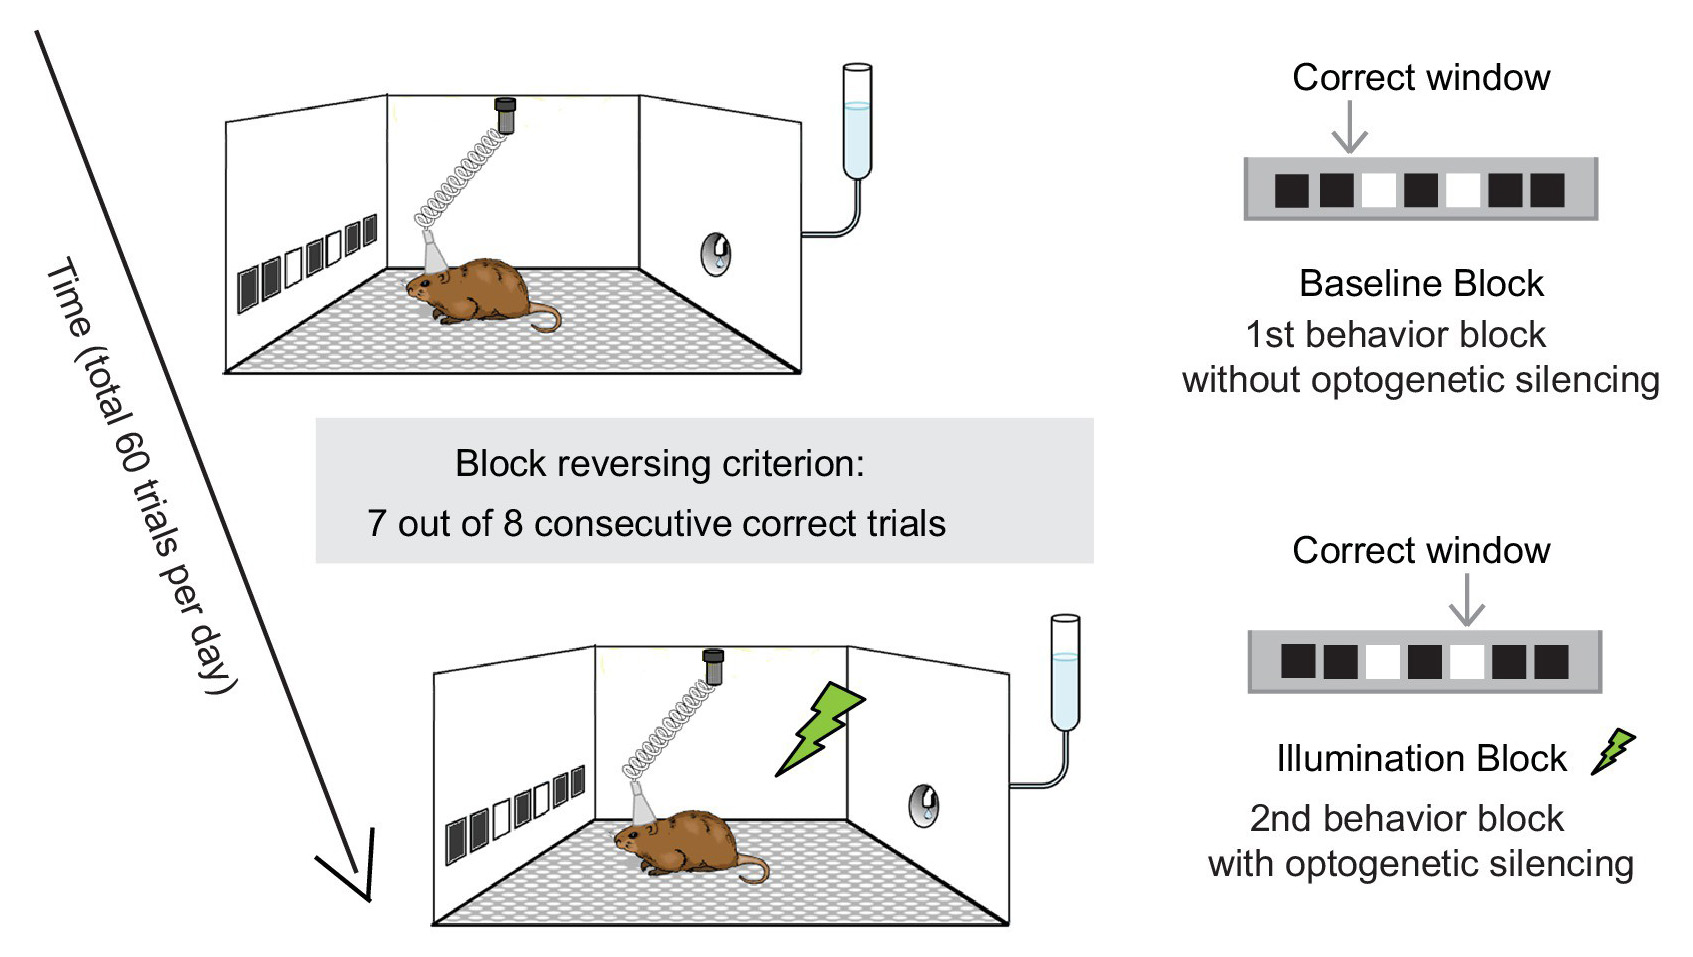
\includegraphics[width=15cm]{task-schematic.jpg}
	\caption{behaivorbox schematic}
	\label{fig:behaivorbox schematic}
\end{figure}

\subsection{
	IR Touchscreen}\label{sec:ir-touchscreen}

The IR touchscreen provided a robust measure of the location of any contact with the animal's paws or nose.
The screen was more reliable than either \emph{resistive} or \emph{capacitive} touchscreens, which are much more common in devices like POS systems and mobile phones respectively.

The scientists users interact with the device through command-line manipulation of a ``BehaviorBox'' object in the MATLAB REPL.
This approach provides access to features for easily customizable control of physical components including the infrared touchscreen and LCD display along with speakers, water-ports, lights, essentially anything that can be controlled electronically.
The approach also enables suggestions and autocomplete options for users new to the environment.

\subsection{
	FrameSynx Toolbox}\label{sec:framesynx-toolbox}

The FrameSynx toolbox for MATLAB was built to synchronize continuous image acquisition with experiments conducted in the neuroscience laboratory setting.
While the experiments are conducted in separate software (and potentially on a different computer), FrameSynx listens for messages to start/stop the experiment, start a trial, etc. and responds accordingly by controlling one or multiple cameras and illumination devices, and synchronizing this information with the data acquired.
The major contribution to the ``Behavior Box'' package, and also to later image processing packages is the procedure for definition and storage and of experimental data files, which will be touched on briefly in {[}@sec:data-file{]}

\subsection{Using Computer Vision to track Position and Orientation}\label{sec:using-computer-vision-to-track-position-and-orientation}

\subsection{Mouse in a Bowl}\label{mouse-in-a-bowl}

A webcam-based motion tracking box constructed to analyze the movement of our unilaterally lesioned PD mouse model.
Video is recorded at 15 frames per second and processed on-line or off-line using a function written in MATLAB.
Briefly, this function converts each frame to a black and white image (logical matrix), uses morphological filtering functions to isolate the mouse (remove mouse excrement) and identify its body (remove the tail), then finds the center of mass in cartesian coordinates (maximum center of projection on x- and y-axes), and the rostral-caudal orientation measured in degrees off the x-axis.
Orientation is determined by the index of maximum of a radon transform of the binary image.
Processing is accomplished at a rate of 15-16 fps, using a single core, or 64 fps using parallel processing on a quad-core processor with multi-threading enabled.
The advantage of this apparatus over the virtual-reality system is that it allows free movement of an untrained mouse, with real-time movement metrics at nearly the same rate as the spherical treadmill.

\begin{figure}[htb]
	\begin{minipage}[t]{0.32\linewidth}\centering
		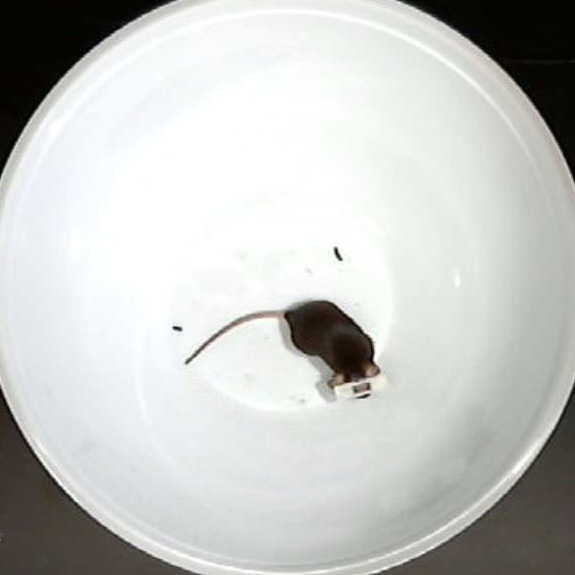
\includegraphics[width=4cm]{01raw.jpg}
		\centerline{(a)}
	\end{minipage}
	\hfill
	\begin{minipage}[t]{0.32\linewidth}\centering
		
\includegraphics[width=4cm]{02black-and-white.jpg}
		\centerline{(b)}
	\end{minipage}
	\begin{minipage}[t]{0.32\linewidth}\centering
		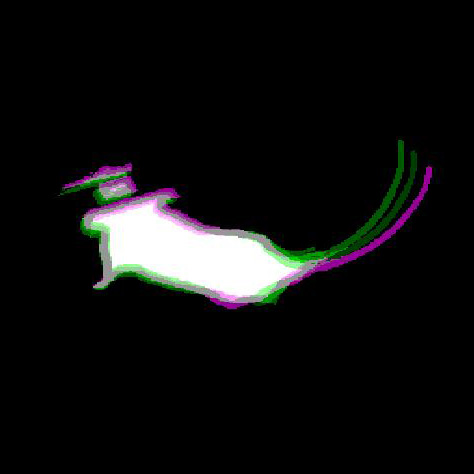
\includegraphics[width=4cm]{03twoframes.jpg}
		\centerline{(c)}
	\end{minipage}
	\caption{
		Automated animal Tracking for ``Mouse in a bowl'' type experiments (a) Raw frame of video being tracked;
		(b) area of detected mouse; (c) overlay of 3 consecutive frames of mouse between each}
	\label{fig:Sampling}
\end{figure}

\begin{figure}[htb]
	\begin{minipage}[t]{0.24\linewidth}\centering
		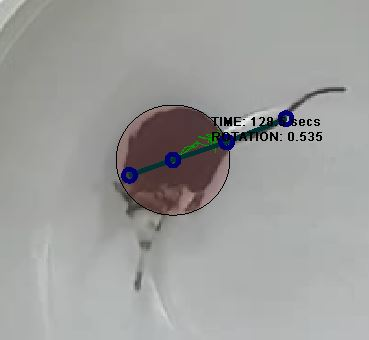
\includegraphics[height=3cm]{07mousedata1close.jpg}
		\centerline{(a)}
	\end{minipage}
	\hfill
	\begin{minipage}[t]{0.24\linewidth}\centering
		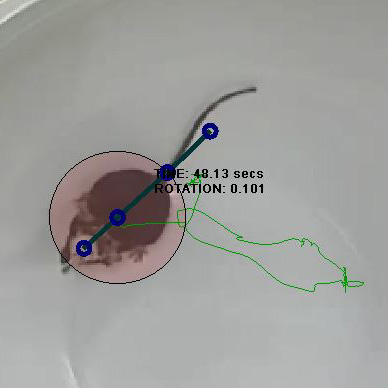
\includegraphics[width=3cm]{06mousedata1.jpg}
		\centerline{(b)}
	\end{minipage}
	\begin{minipage}[t]{0.24\linewidth}\centering
		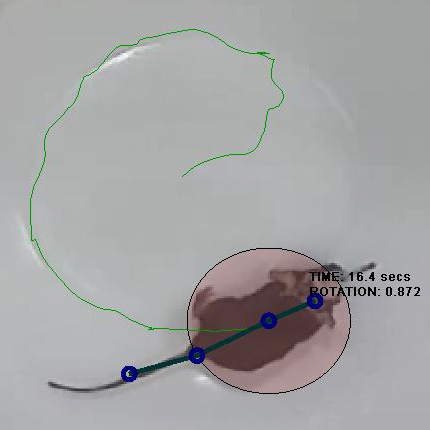
\includegraphics[width=3cm]{08mousedata2.jpg}
		\centerline{(c)}
	\end{minipage}
	\begin{minipage}[t]{0.24\linewidth}\centering
		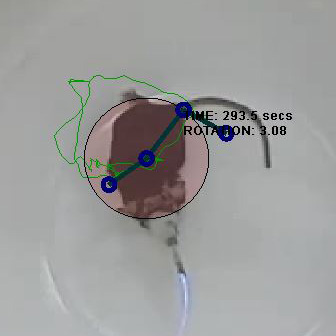
\includegraphics[width=3cm]{09mousedata1fiberon1.jpg}
		\centerline{(d)}
	\end{minipage}
	\caption{
		Automated animal Tracking for ``Mouse in a bowl'' type experiments: (a-d) video overlay showing tracked points} \label{fig:Sampling}
\end{figure}

\subsection{Spherical Treadmill}\label{spherical-treadmill}

A virtual reality system was assembled, adopting methods from the Harvey lab lab {[}@harvey\_intracellular\_2009{]}.
This system allows placement of a head-restrained mouse on an 8-inch diameter polystyrene foam ball supported by a cushion of compressed air, surrounded by a toroidal projection screen.
Ball rotation is tracked with two optical computer mice placed orthogonal to each other.
Movement vectors are fed into a virtual-reality engine that updates the image projected onto a toroidal screen surrounding the ball, simulating movement through any arbitrary virtual world.
Movement vectors are recorded as an arbitrarily scaled translation in the mouse-relative X and Y axes and rotation around the Z axis, at approximately 30 ms intervals.
This behavioral apparatus has the advantage of allowing trivial measurement of the mouse's movement ability while the mouse is head-fixed.
The disadvantage is the time and potential confounds involved with training individual mice to use the system.

\begin{figure}[htb]
	\begin{minipage}[t]{0.32\linewidth}\centering
		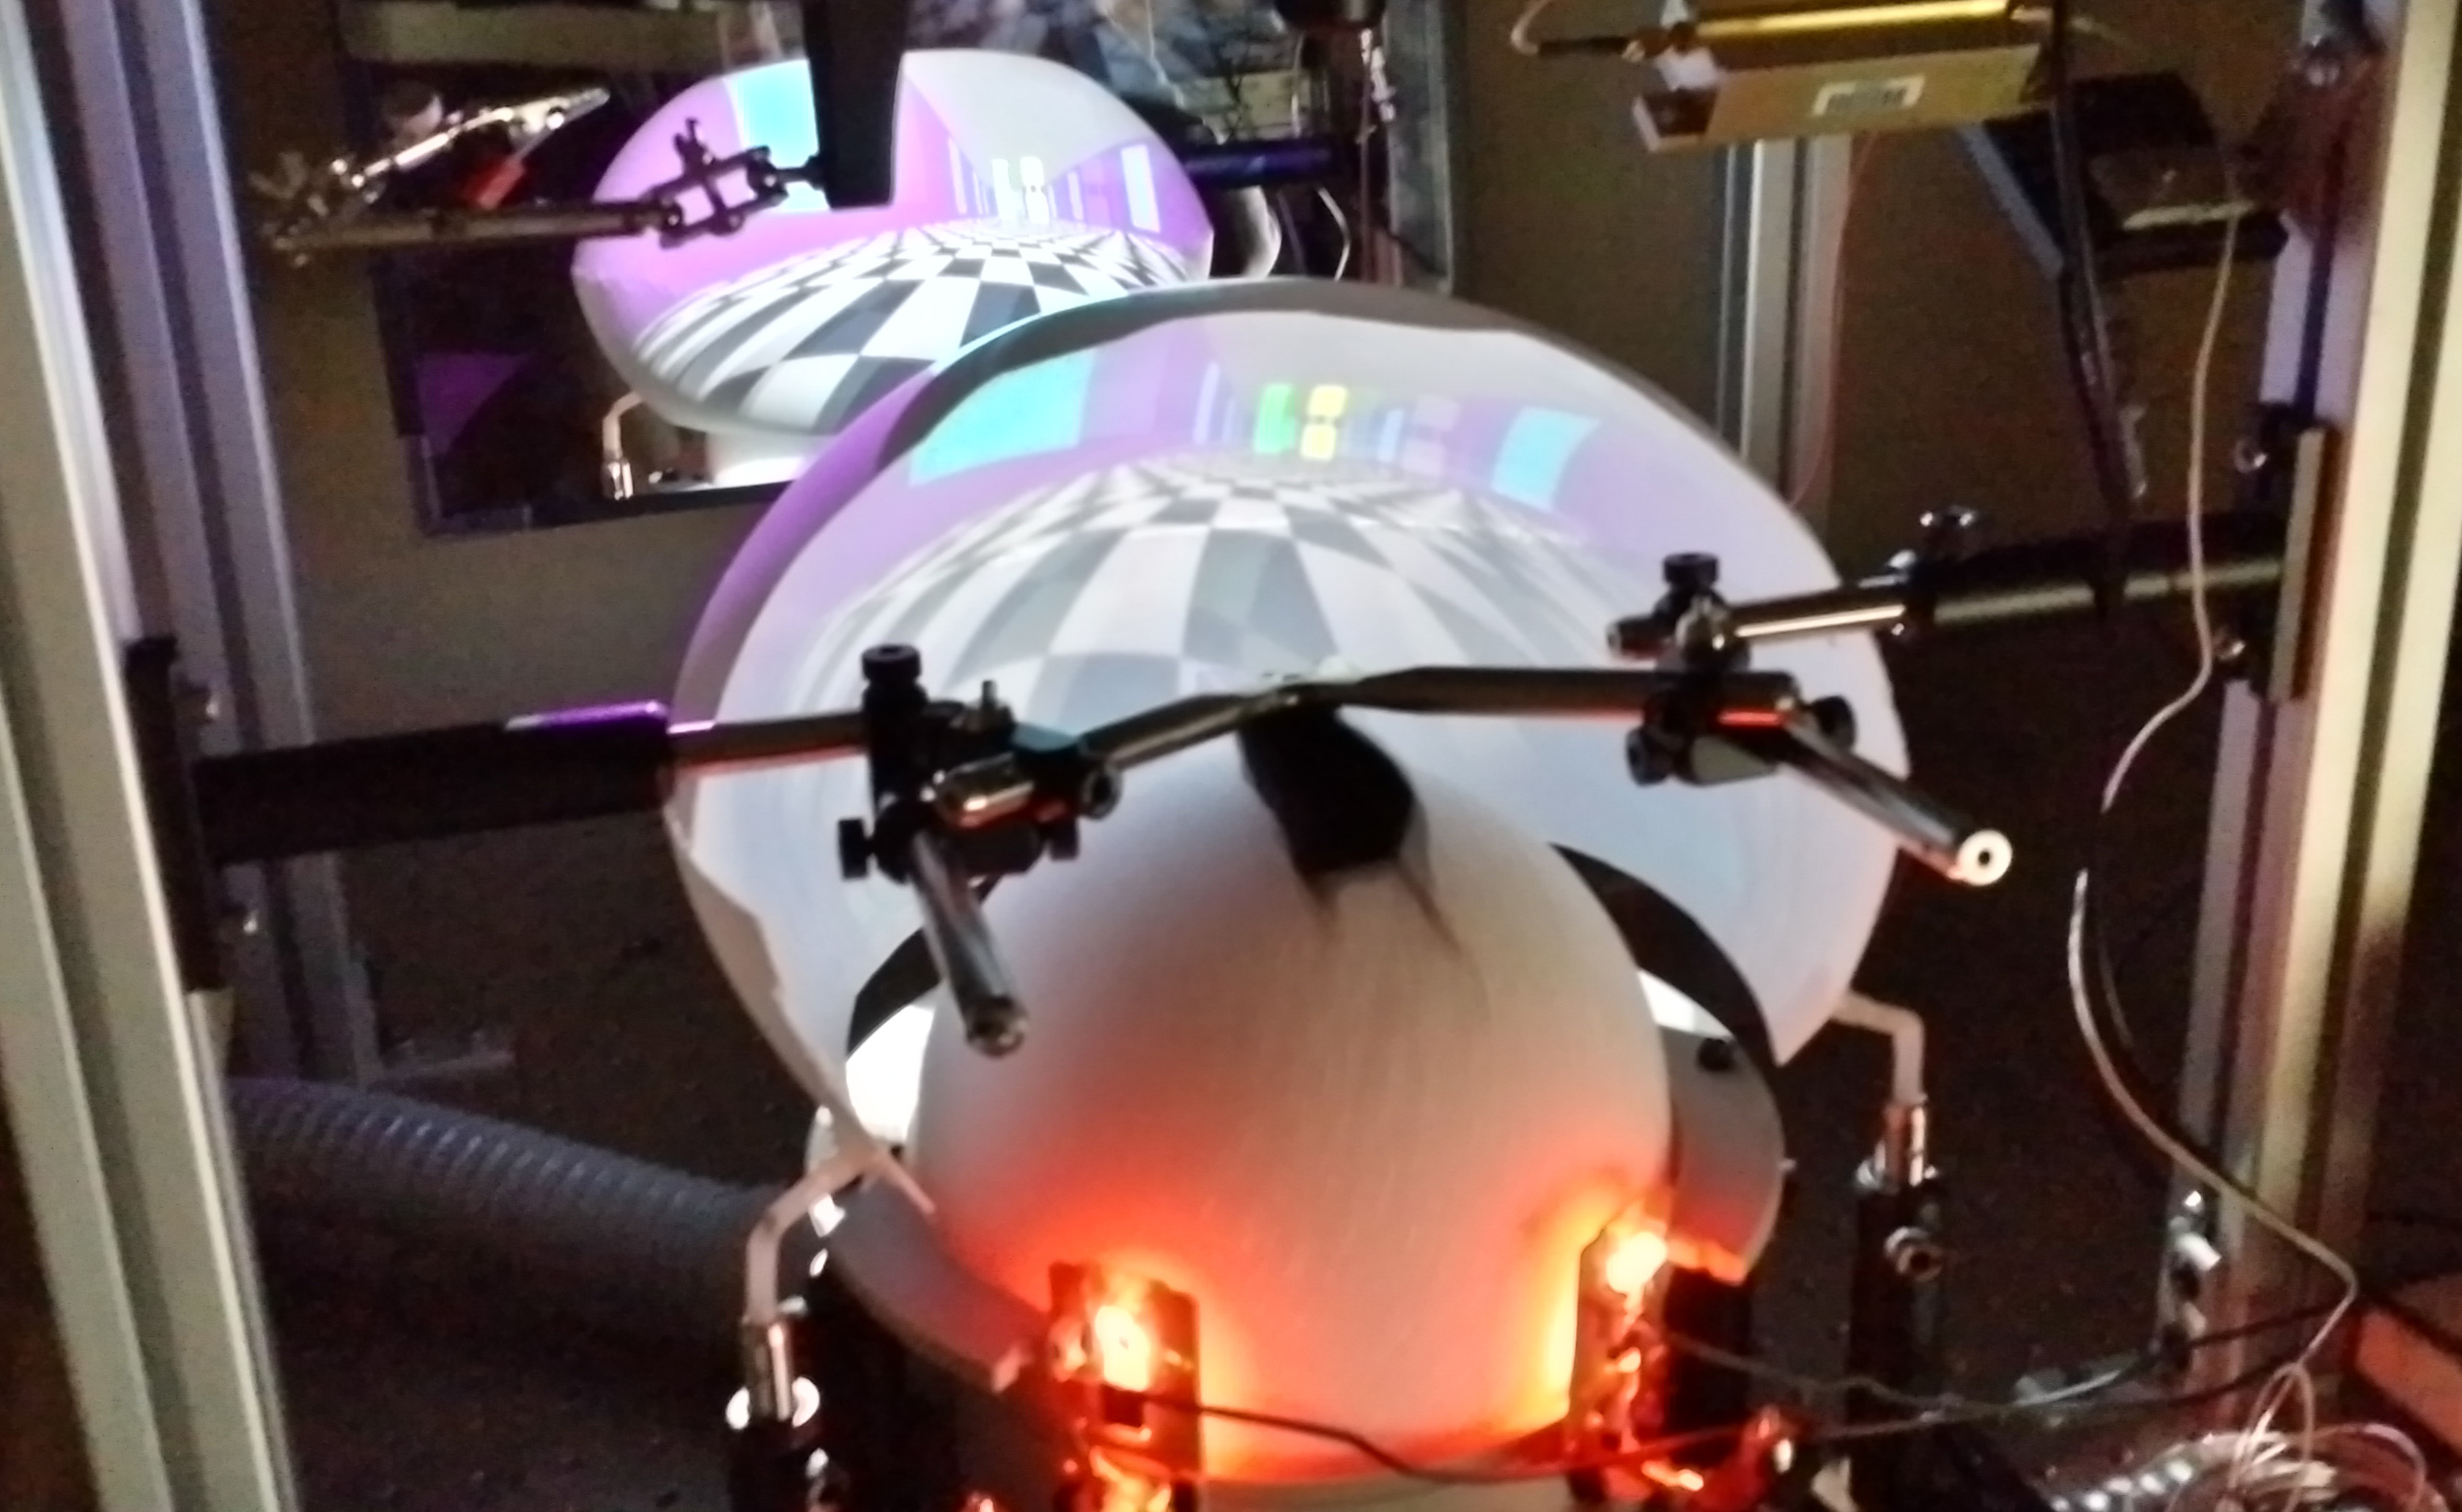
\includegraphics[height=3.5cm]{01-treadmill-mouse-running.jpg}
		\centerline{(a)}
	\end{minipage}
	\hfill
	\begin{minipage}[t]{0.15\linewidth}\centering
		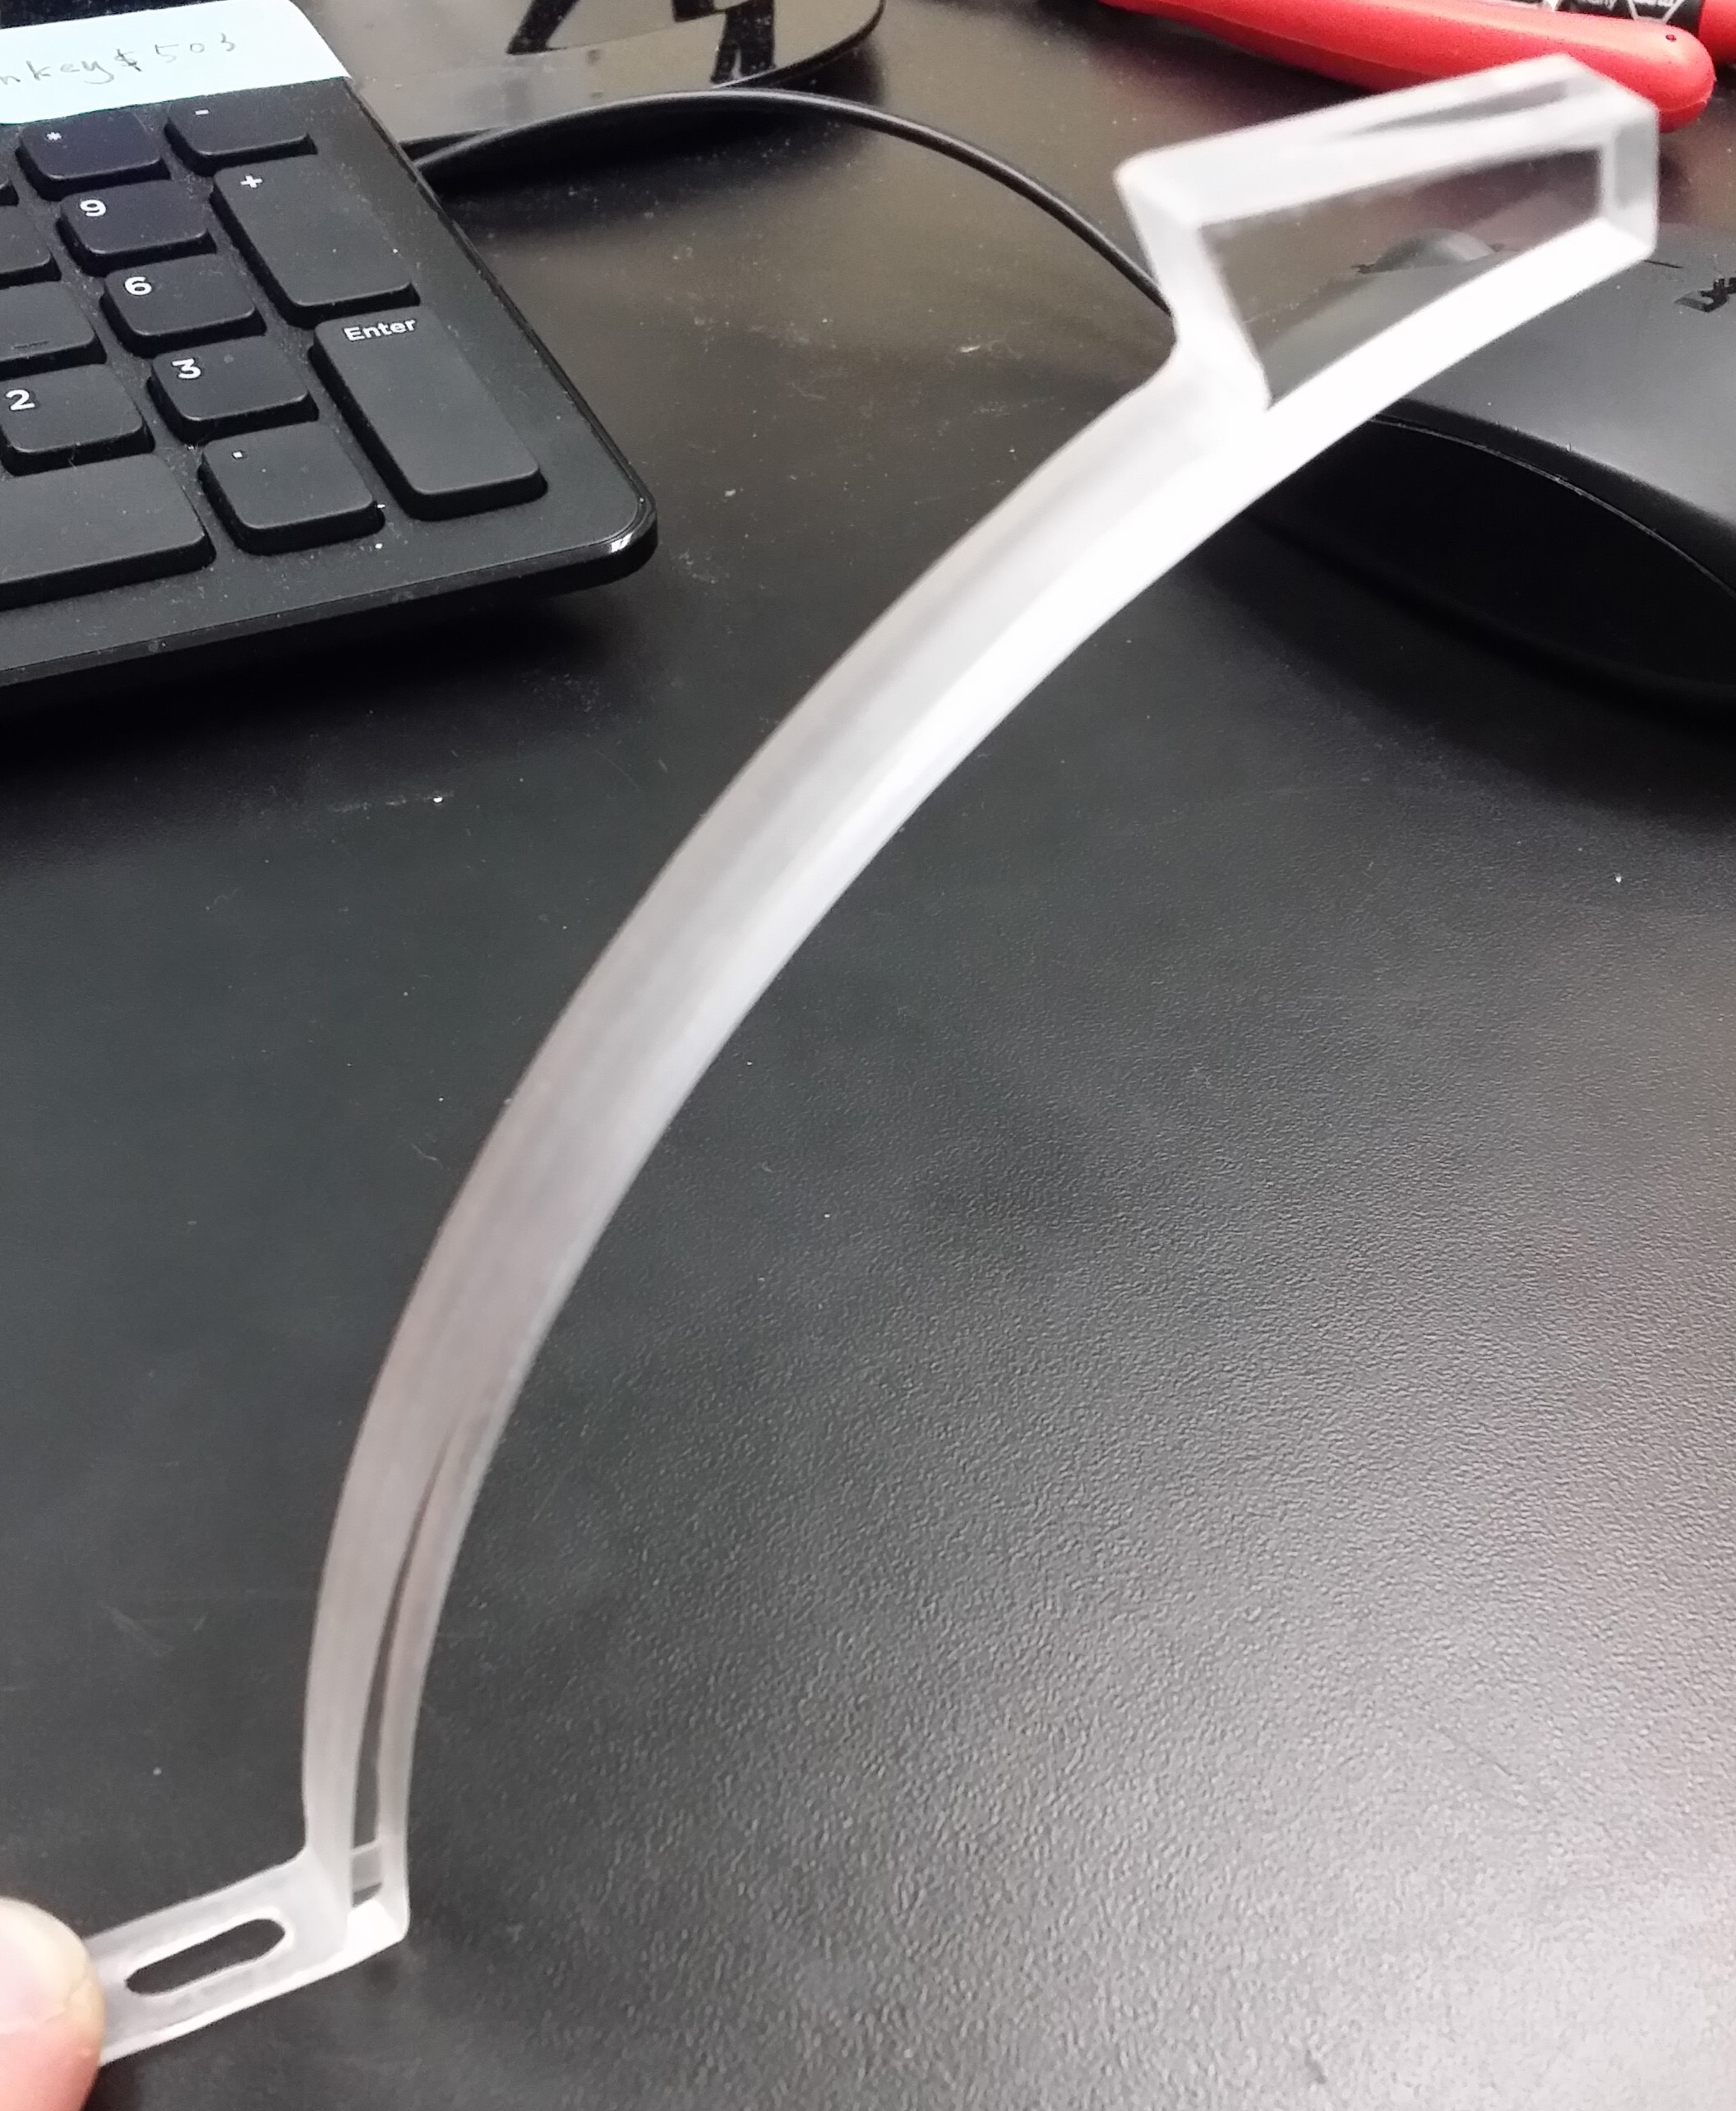
\includegraphics[height=3.5cm]{01-water-port.jpg}
		\centerline{(b)}
	\end{minipage}
	\begin{minipage}[t]{0.45\linewidth}\centering
		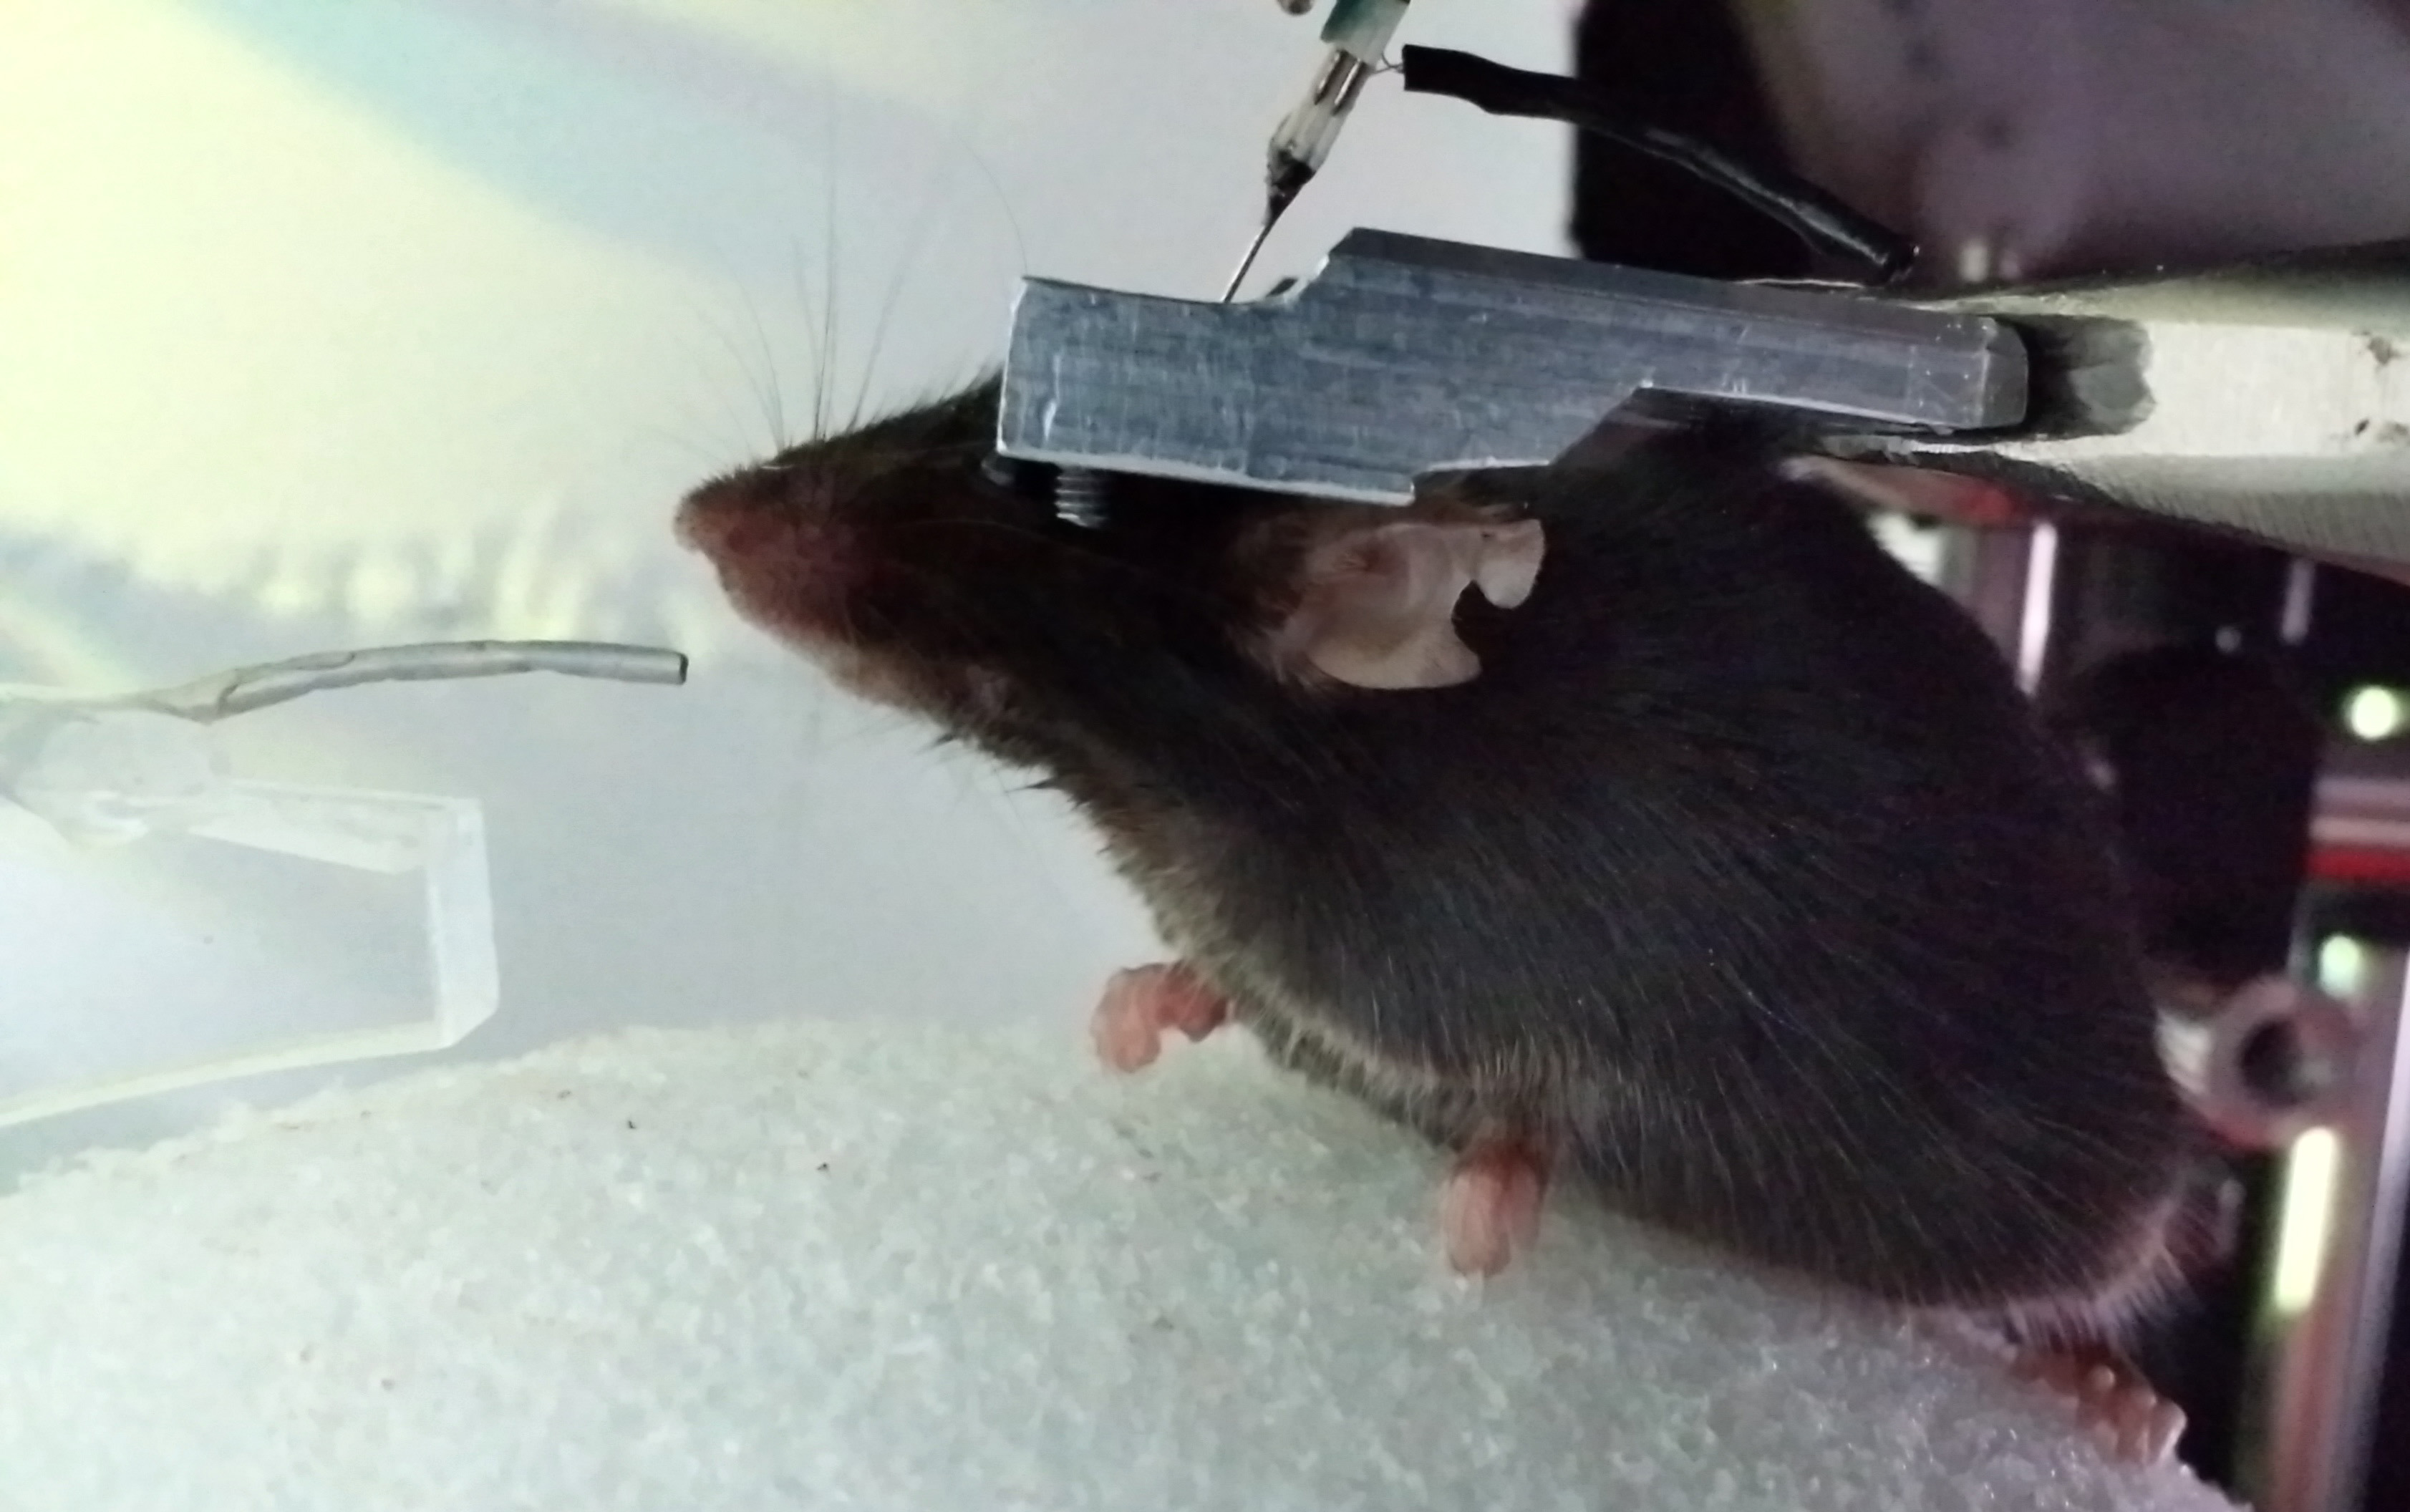
\includegraphics[height=3.5cm]{03-water-delivery-zoom.jpg}
		\centerline{(c)}
	\end{minipage}
	\caption{
		Spherical treadmill (a) Mouse running on a treadmill equpipped with virtual reality;
		(b) water port; (c) application of the water delivery system }
	\label{fig:Spherical treadmill}
\end{figure}

\subsection{
	Headplate Holder}\label{headplate-holder}

\begin{figure}[htb]
	\begin{minipage}[t]{0.32\linewidth}\centering 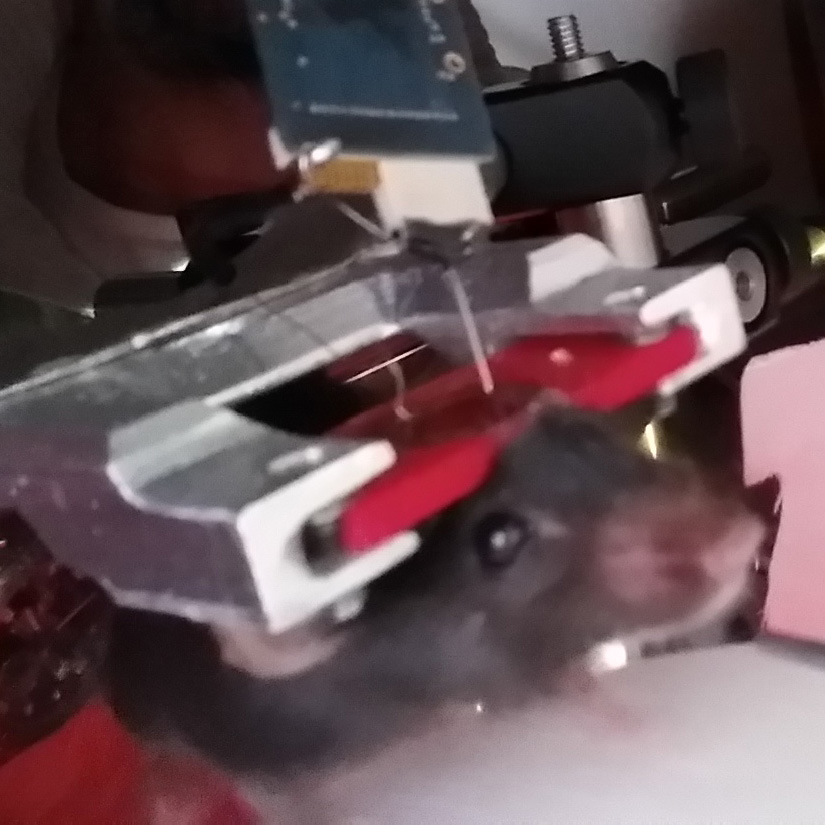
\includegraphics[width=4.5cm]{photo-front.jpg} \centerline{(a)}
	\end{minipage}
	\hfill
	\begin{minipage}[t]{0.32\linewidth}\centering 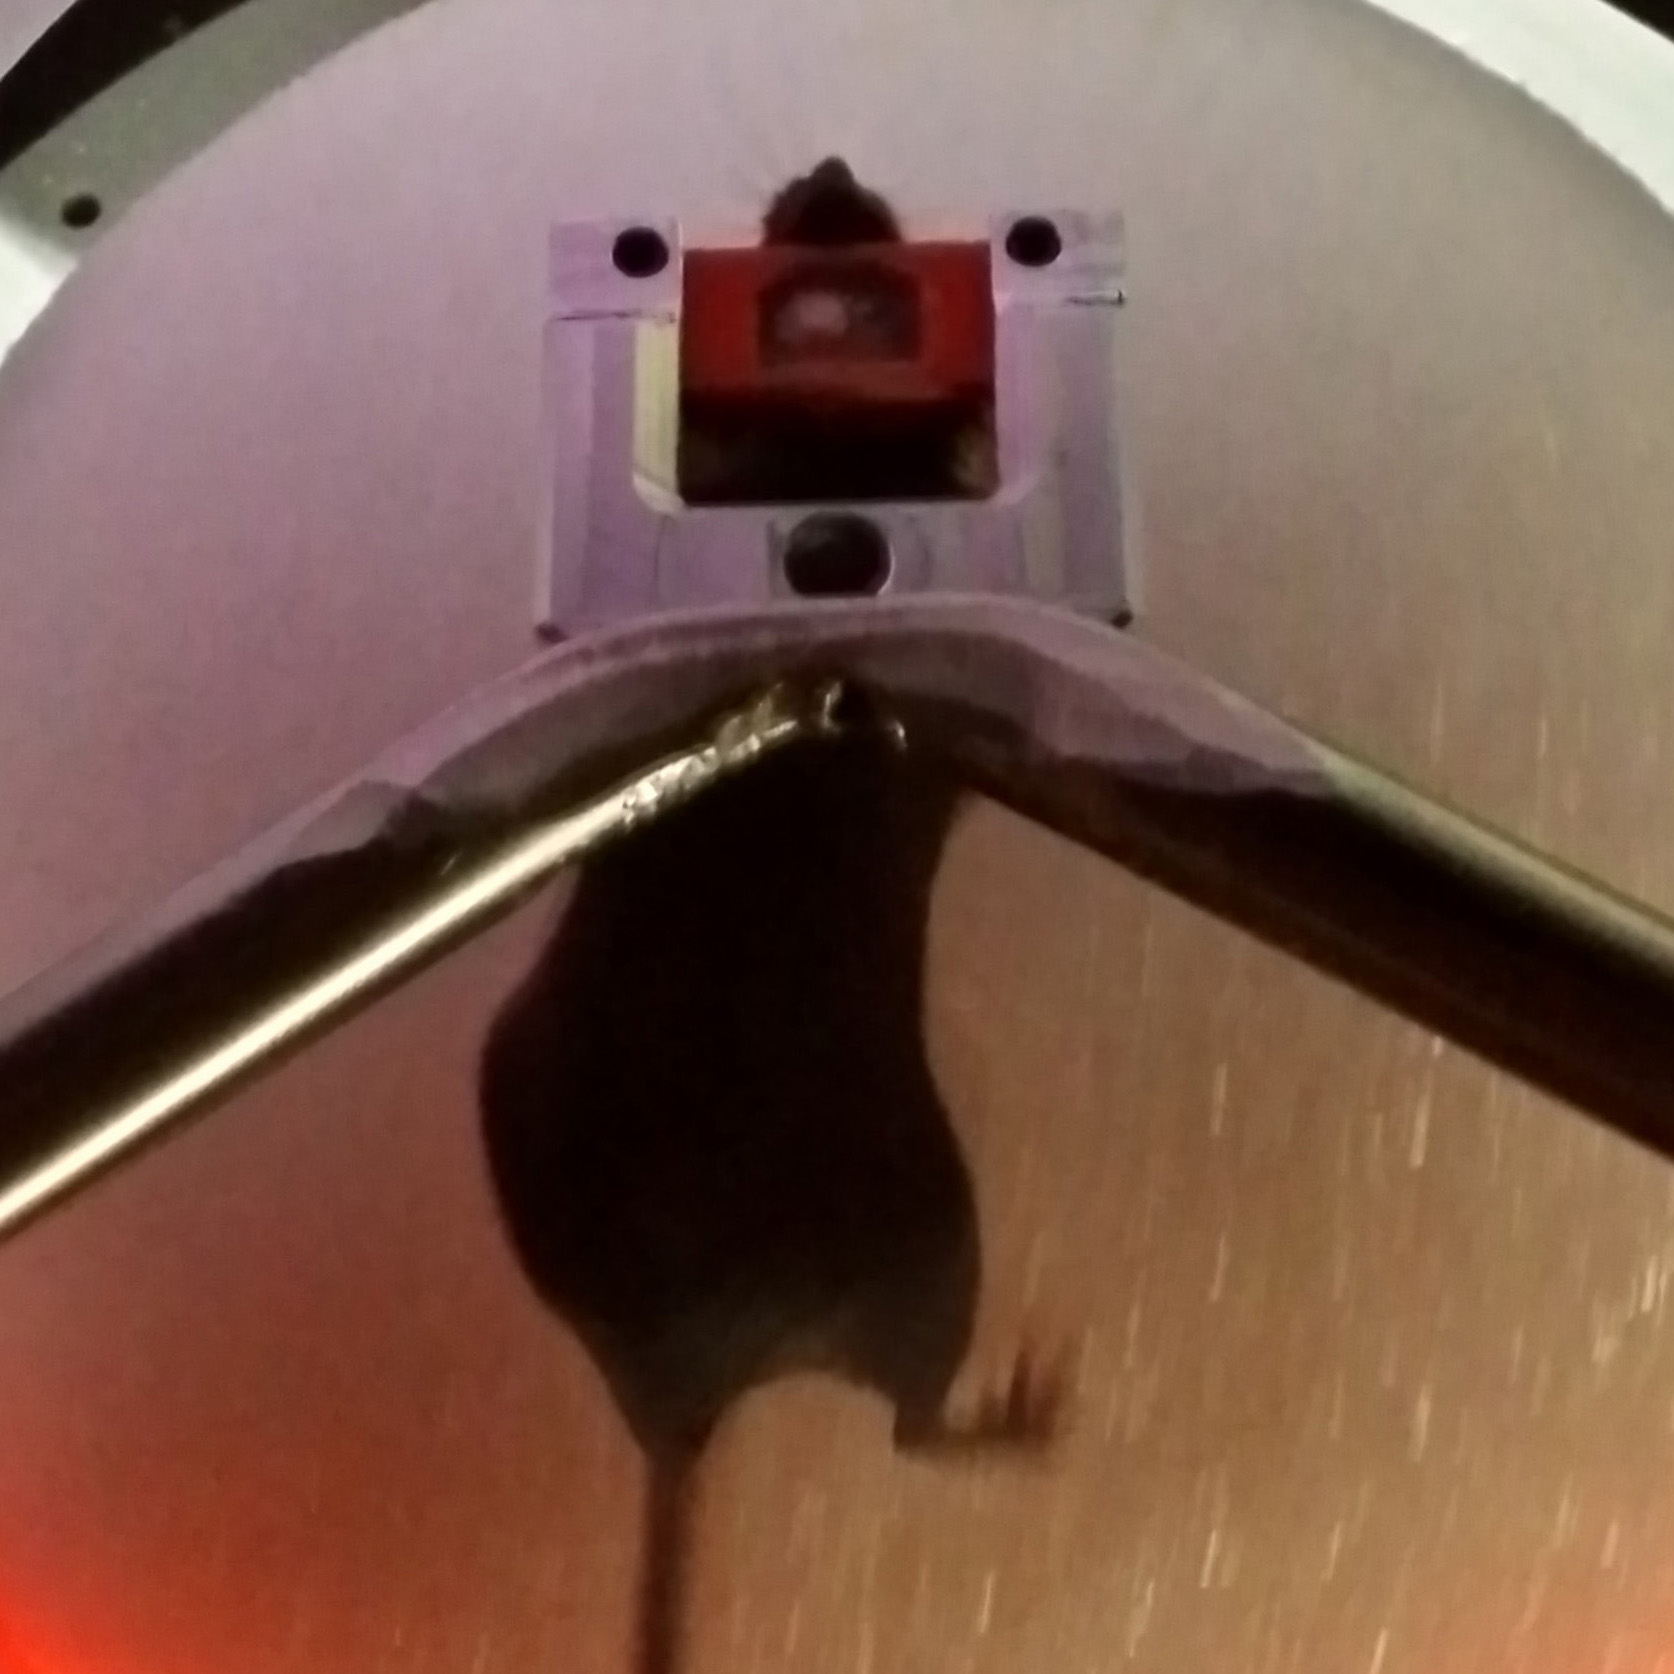
\includegraphics[width=4.5cm]{photo-top.jpg} \centerline{(b)}
	\end{minipage}
	\begin{minipage}[t]{0.32\linewidth}\centering 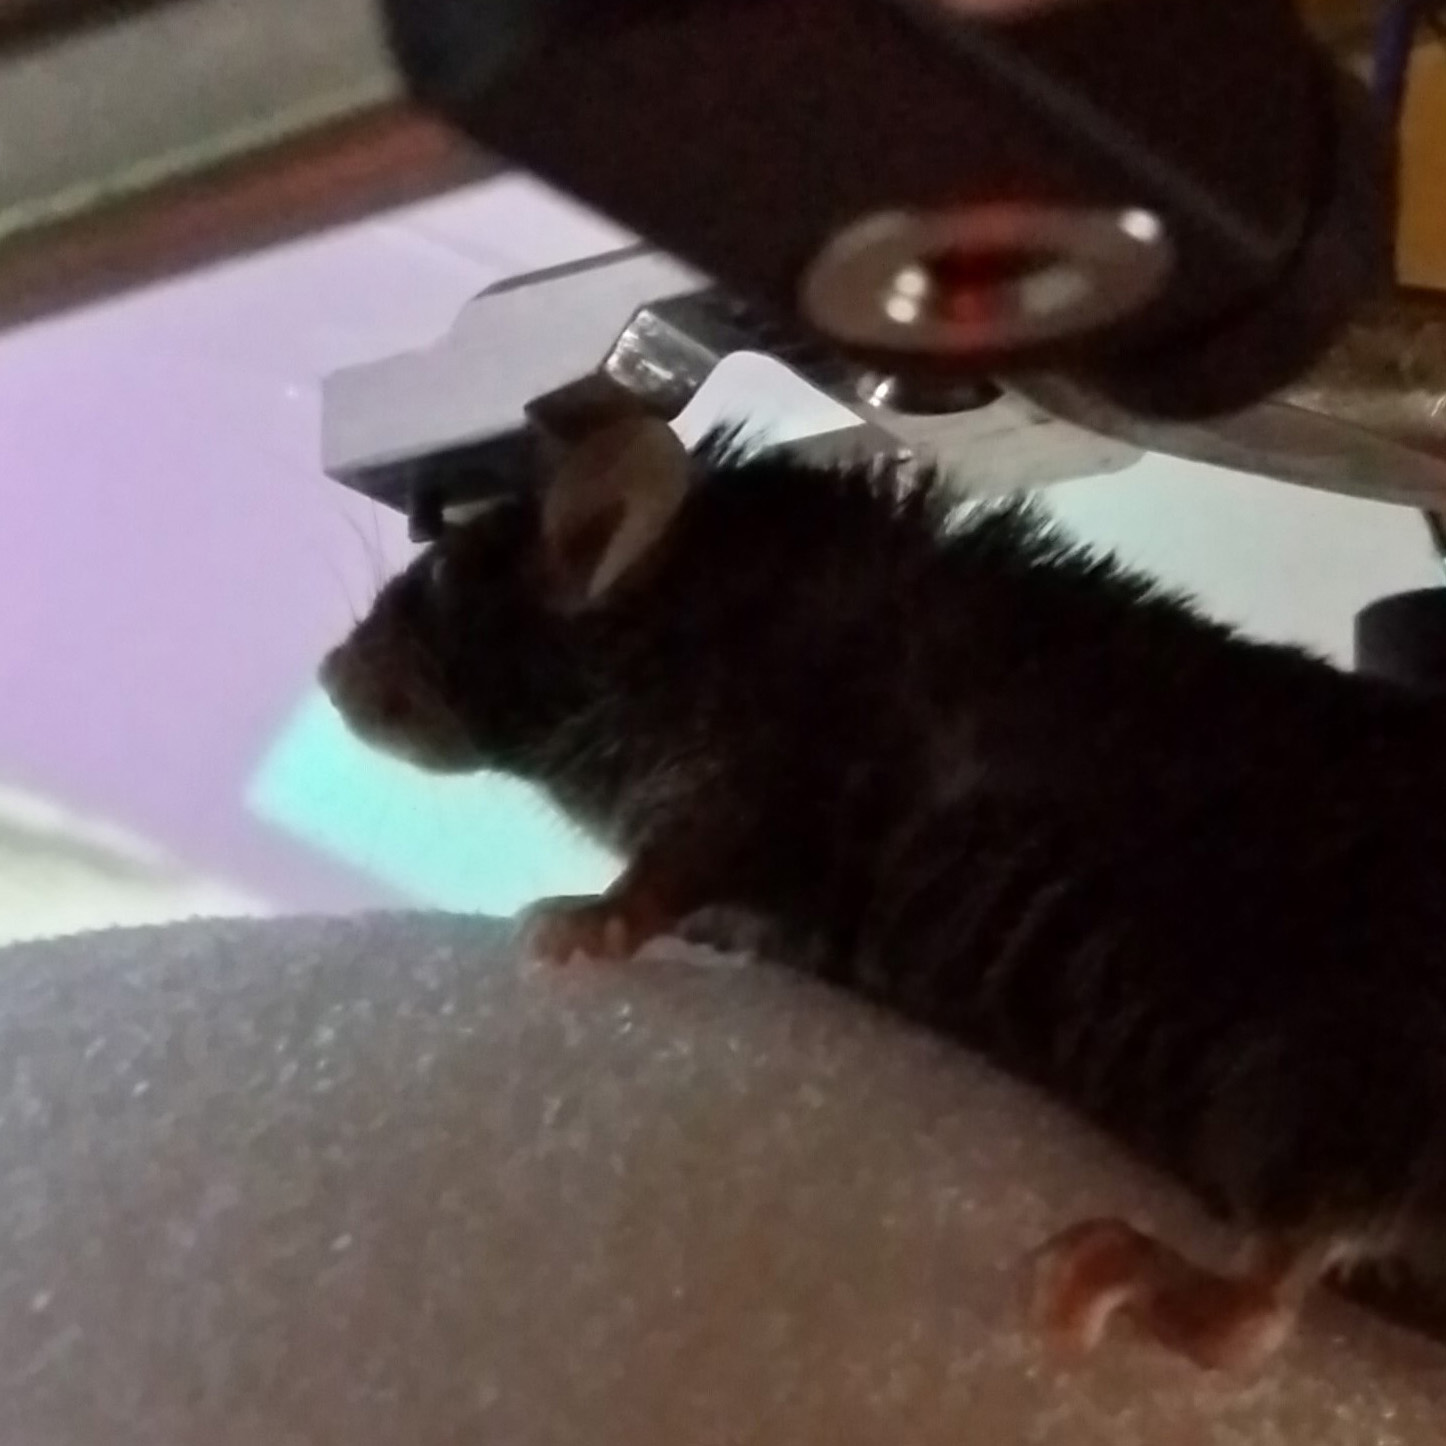
\includegraphics[width=4.5cm]{photo-bottom.jpg} \centerline{(c)}
	\end{minipage}
	\caption{Headplate holder (a) front view;
		(b) top view; (c) bottom view}
	\label{fig:Spherical treadmill}
\end{figure}

\subsection{
	Motion Sensors}\label{motion-sensors}

Motion sensing was implemented using a linux computer and standard mice at first, and later using precision laser navigation sensors for ``gaming'' mice and custom firmware written to work with any arduino-compatible microcontroller.

\subsection{
	Generic USB Computer Mouse with Minimal Linux}\label{generic-usb-computer-mouse-with-minimal-linux}

Run ``mouse\_relay.py'' on any computer running linux to send xy-data from 2 USB optical computer mice to another computer over an RS-232 serial-port connection.
The receiving computer (in this implementation) uses MATLAB to read the values and translate the xy-values from 2 mice on the surface of a sphere into 3 values corresponding to rotation of that sphere around 3 orthogonal axes (XYZ) with their origin at the sphere's center.

RECEIVING FUNCTIONS: The MATLAB class that receives the serial input (xy-values from both mice) is called ``VrMovementInterface''

The MATLAB function that translates the double-stream of xy-values from the sphere's surface into rotation around its center is called ``moveBucklin.m'' and is located in the VIRMEN ``movements'' folder.

SERIAL FORMAT: XY-Values are transmitted in `packets' using an ascii formatted string terminated by a newline.
Each packet contains the Sensor Number (s) that the reading is coming from, followed by the X-Value (dx), then the Y-Value (dy).
The python code looks like the following:

A single reading is received at the other end of the serial connection looking something like the following:

\begin{quote}
	s1x34y-3
\end{quote}

\subsection{Navigation Sensor Chip with Arduino}\label{navigation-sensor-chip-with-arduino}

The system was later improved.
%\begin{Shaded}%\begin{Highlighting}[]%\NormalTok{> datastring = s + }\StringTok{'x'}\NormalTok{+dx + %}\StringTok{'y'}\NormalTok{+dy + %}\StringTok{'}\CharTok{\textbackslash{}n}\StringTok{'}%\end{Highlighting}%\end{Shaded}
Works with ADNS library to pass {[}dx,dy{]} measurements from two ADNS-9800 laser mouse sensors (placed 45-degrees apart on surface of Styrofoam ball).

\begin{figure}[htb]
	\begin{minipage}[t]{0.45\linewidth}\centering
		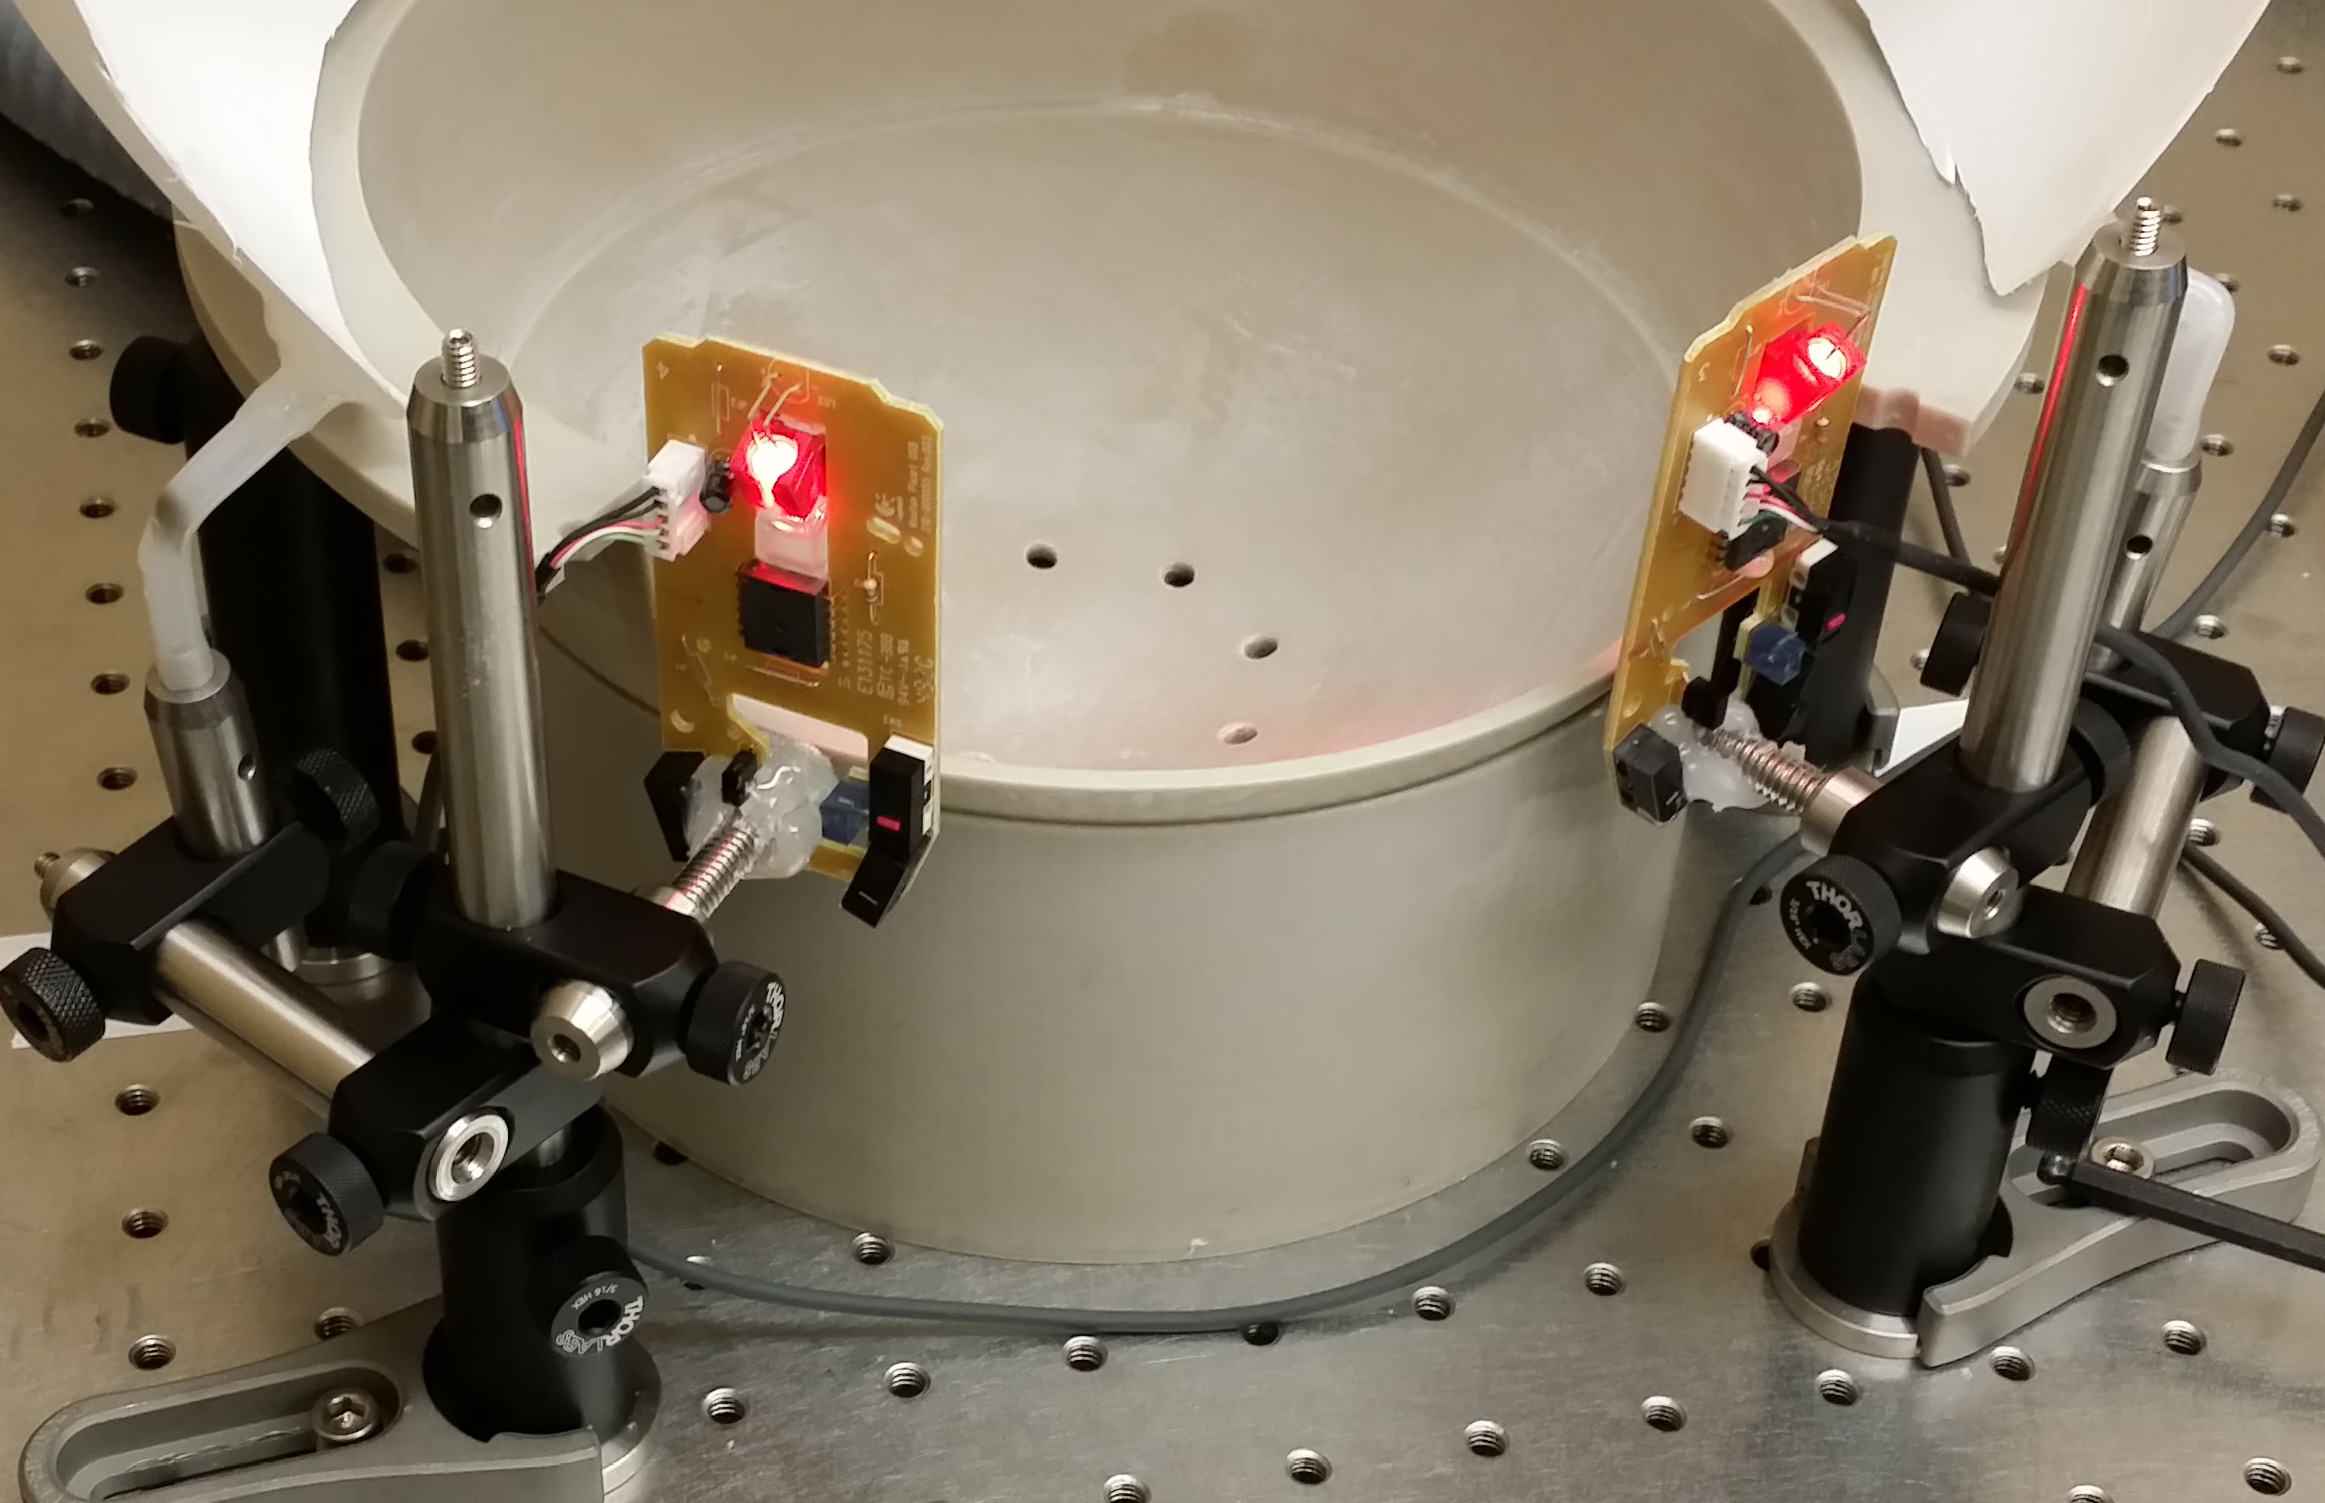
\includegraphics[height=4.5cm]{2_body/figures/01-motion-sensors-installed.jpg}
		\centerline{(a)}
	\end{minipage}
	\hfill
	\begin{minipage}[t]{0.45\linewidth}\centering
		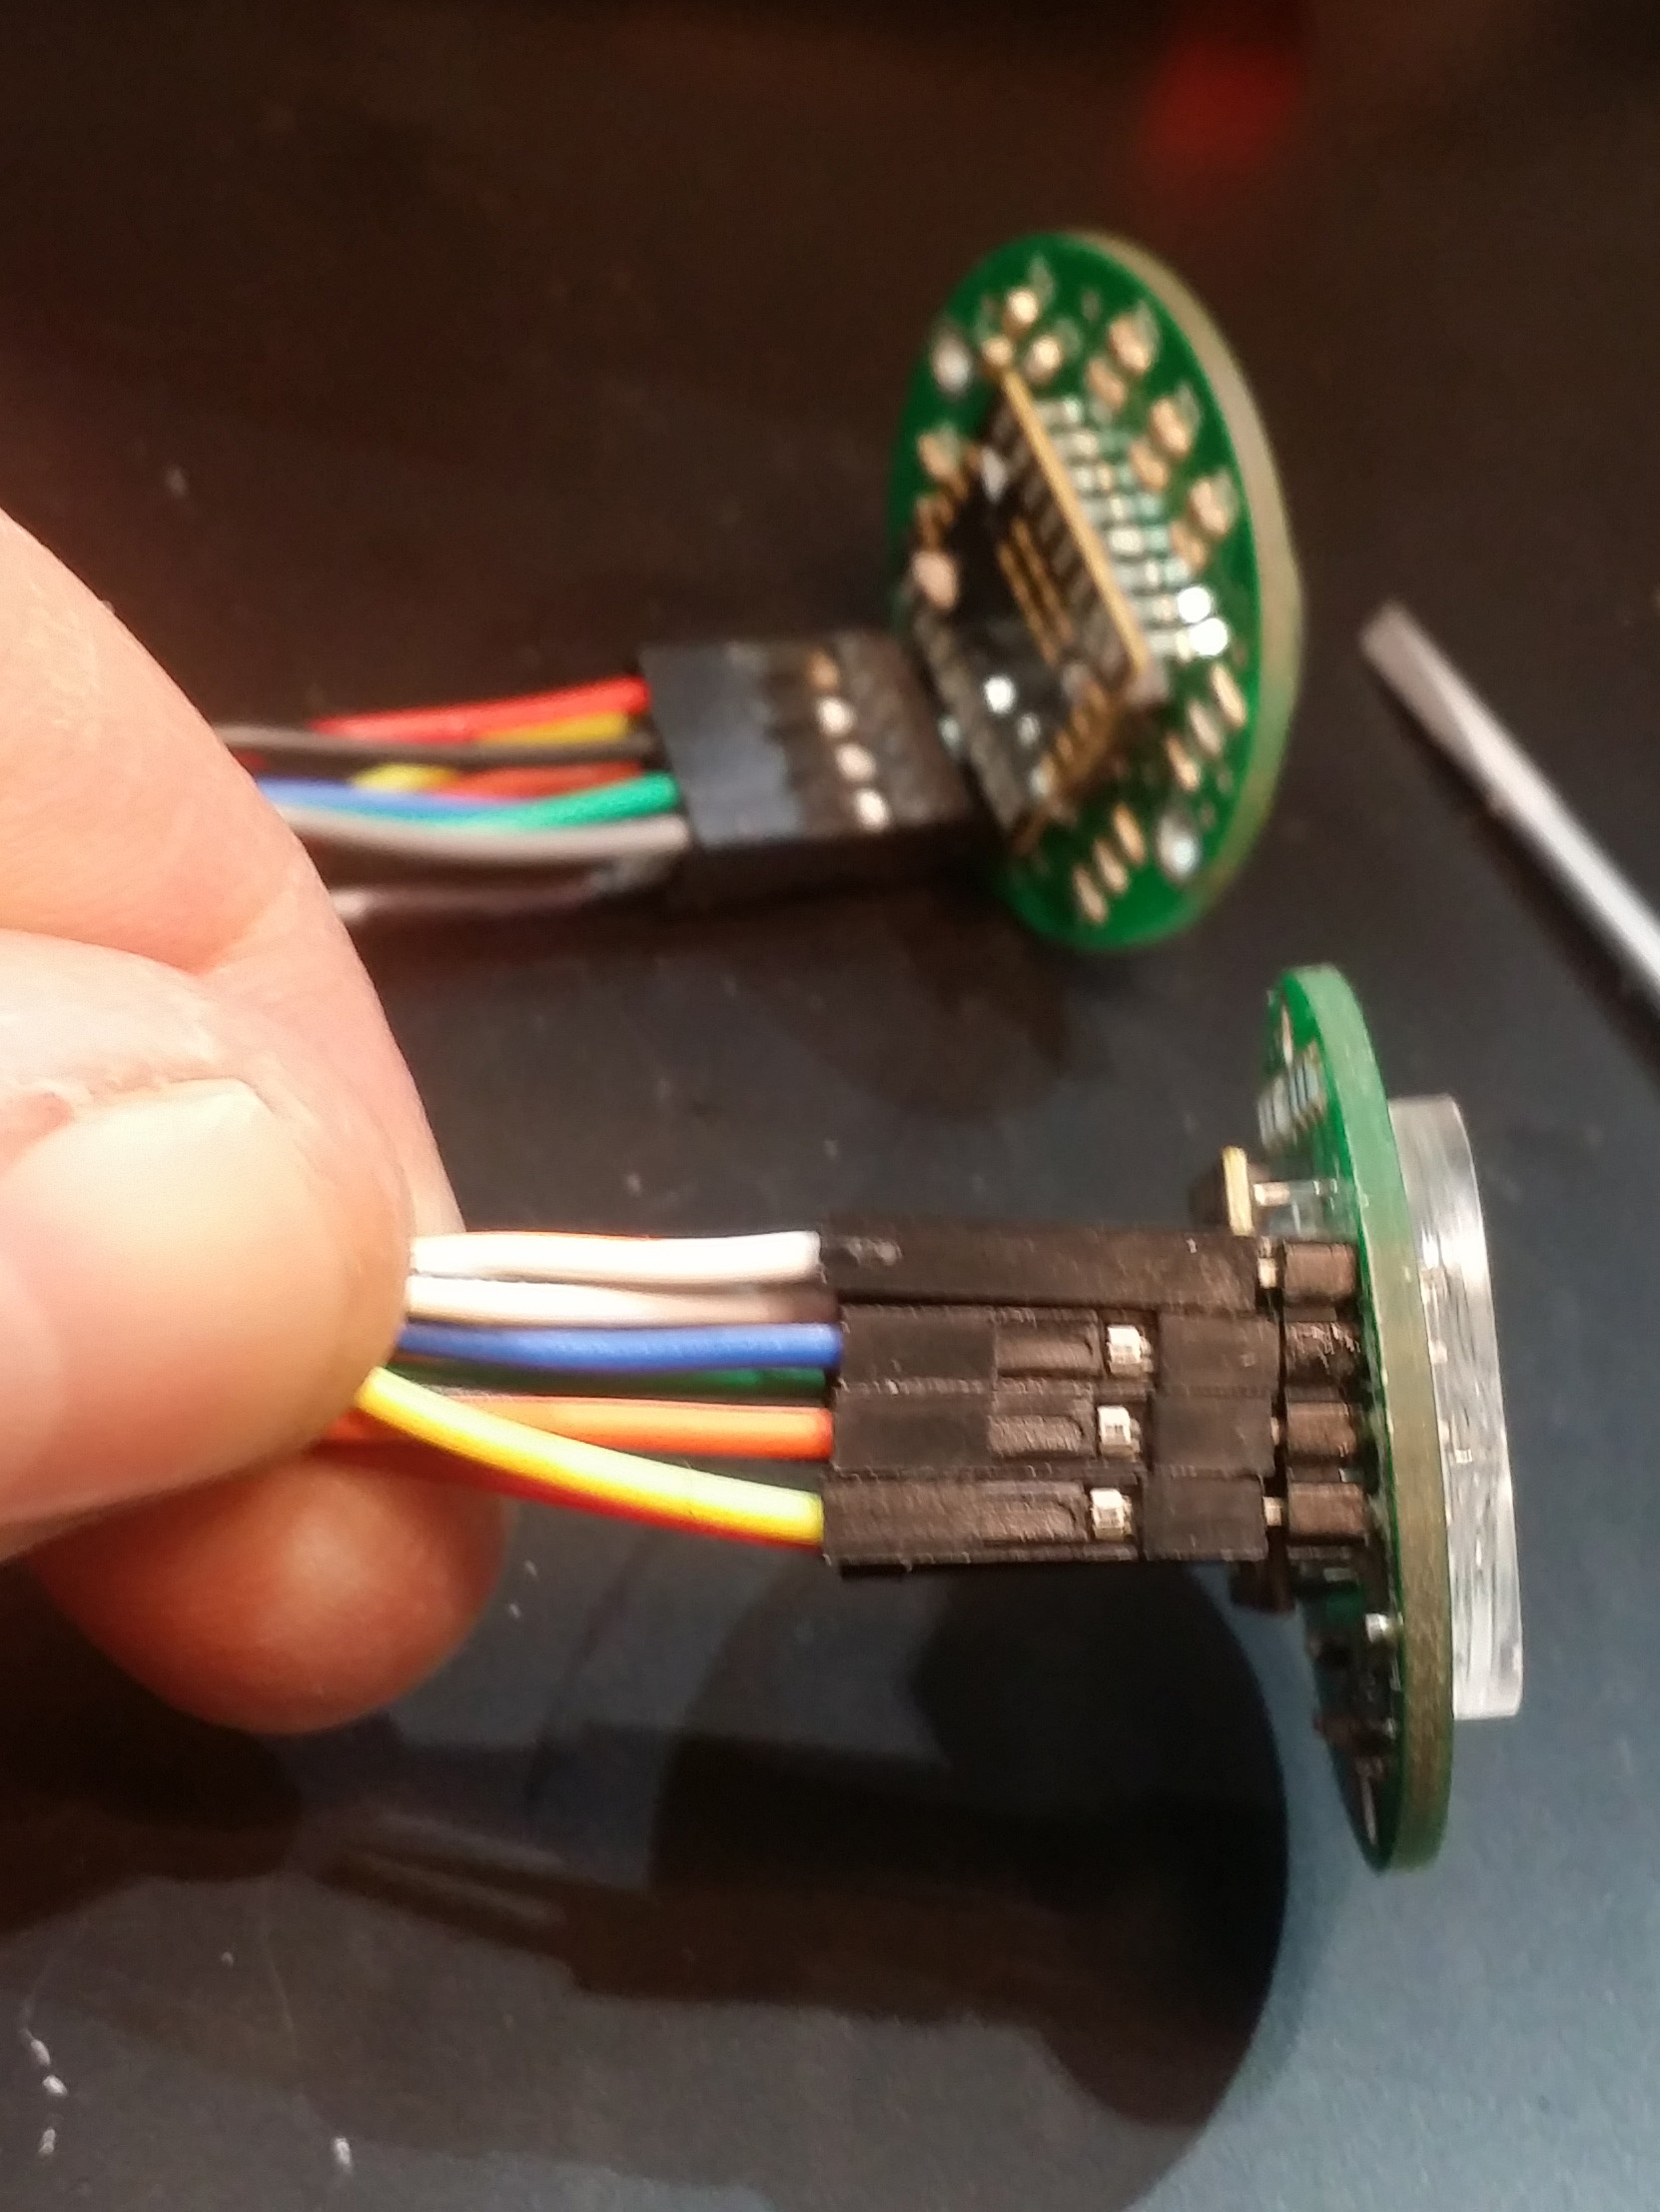
\includegraphics[height=4.5cm]{2_body/figures/02-motion-sensors.jpg}
		\centerline{(b)}
	\end{minipage}
	\begin{minipage}[t]{\linewidth}\centering
		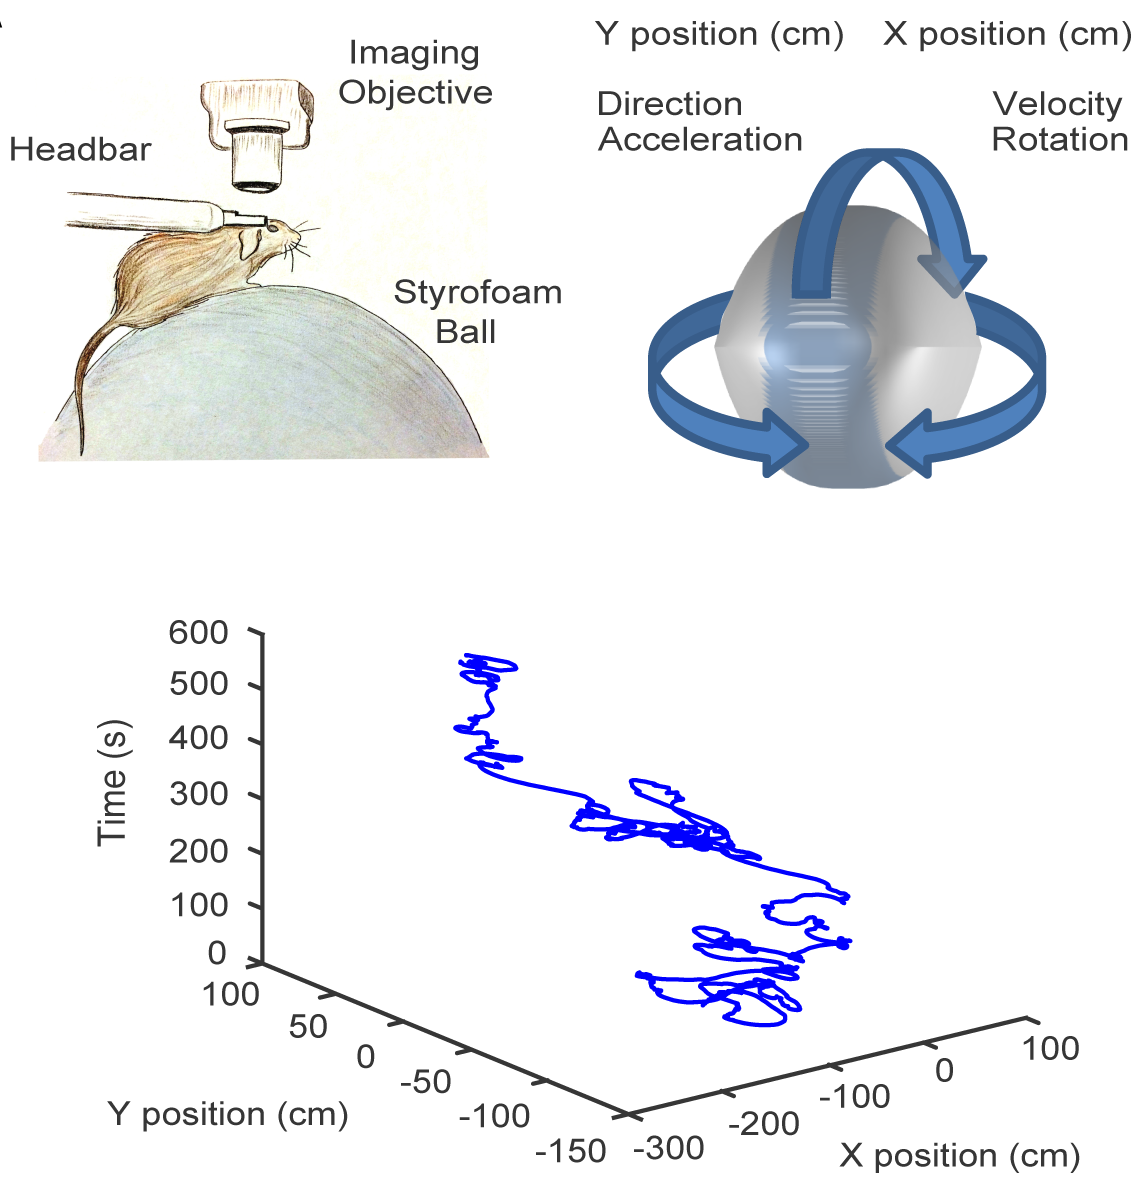
\includegraphics[height=7cm]{2_body/figures/Striatum_Figure2.png}
		\centerline{(c)}
	\end{minipage}
	\caption{
		Motion sensors (a) mention sensors installed;
		(b) motion sensors; (c) tracking mouse movement}
	\label{fig:motion sensors}
\end{figure}

\section{
  Microscopes}\label{microscopes}

This section describes the background in microscopy in the neurosciences, and also how it relates to imaging in healthcare and electrophysiology in neuroscience.
It will also describe the basic elements necessary for the construction of a microscope in a laboratory where calcium imaging in an animal is available.
It will also refer to later sections which cover the design and construction of mechanical elements for animal handling and optical access (i.e.~the headplate and a chronic optical window).

\subsection{
	Background: Brain Imaging and Microscopy in Neuroscience}\label{background-brain-imaging-and-microscopy-in-neuroscience}

Optical imaging has traditionally involved wide-field imaging or two photon imaging, each with their own distinctive advantages and disadvantages.
In recent years, two photon microscopy has been a preeminent choice for imaging in tissue, because of its high spatial resolution, and tissue penetrating features.
Two photon calcium imaging has been broadly applied to individual cells or subcellular components of neurons including spines and axons.

Because two photon microscopy uses a scanning mechanism, the signal to noise ratio is influenced by the time spent imaging each point, and the spatial resolution is determined by the number of points scanned to obtain each image.
As a result, the size of the imaging field is inversely correlated with the overall temporal resolution while maintaining a relatively high signal-to-noise ratio, thus, two photon calcium imaging is often performed on a small area or on a sparse network of cells, when dynamic responses with high temporal fidelity is necessary.

Wide-field imaging has been used in various forms for several decades and was first used to characterize the functional architecture and hemodynamic responses in brain tissue.
However, this technique has seen a renaissance recently due to its simple instrumentation, relatively inexpensive cost, and the improvements in neural signal indicators.
Optical imaging and two photon microscopy have traditionally been performed in head-fixed preparations, but recent advances have also made it possible to perform wide-field calcium imaging in freely moving animals, through miniaturized and wearable microendoscope systems

While wide-field imaging lacks the spatial resolution to resolve fine subcellular structure or the penetrating properties available with two-photon, it is possible to obtain clear neurites and somatic features, including spike detection

Because a single photon microscope does not rely on scanning features, it can be used to sample a larger field of view without sacrificing sampling rates.
Additionally, recording sessions may be less sensitive to fluorophore bleaching than other techniques, which makes it possible to perform sustained illumination and subsequent imaging for an extended period of time - a desired feature for analyzing neural networks during some behavior paradigms (e.g., repeated trial learning paradigms).
Thus, wide-field imaging offers an advantage if the objective is to simultaneously recording hundreds of neurons in the brain of a living and behaving animal with high temporal fidelity.

\subsection{
	Cameras for Widefield Microscopy}\label{cameras-for-widefield-microscopy}

Traditional widefield microscope or macroscope builds incorporate `scientific grade' cameras.
Compared to cameras built for other markets (e.g.~consumer, industrial, studio, etc.)
, these cameras are often well
tested and certified to offer low or well-characterised noise at
moderate speeds, and a linear photo-response profile.
Unlike consumer or studio cameras which are invaribaly configured for RGB color, they are preferably configured with `monochrome' sensors - essentially identical to the analagous color sensor, without the bayer filter.
Of much greater importance, one must consider the unique connectivity and control interface that scientific cameras come with.
Standards exist, but are typically unique to this segment of the industry, with poorly defined specifications for translation to other electronic communication and connection interface standards, such as those used in studio and broadcast video, or those used with consumer cameras.
The trait that is the most worthy of consideration, however, is the cost.
See @discussion-cost-consumer for details.

The in-vivo instrinsic-signal or fluorescent-dye imaging camera of 1 decade ago had a 0.5``-1'' monochrome CCD sensor with 0.1-1 MegaPixels, a large well-depth, and moderately low noise at speeds around 30 to 60 fps.
Connection was often LVDS, with custom electrial connectors unique to each camera.
A particularly popular and long-running model was the Dalsa 1M30, followed by the 1M60 in later years {[}@takahashi\_vivo\_2006{]}.

\subsection{
	Microscope Construction}\label{microscope-construction}

\begin{figure}[htb]
	\begin{minipage}[t]{0.49\linewidth}\centering 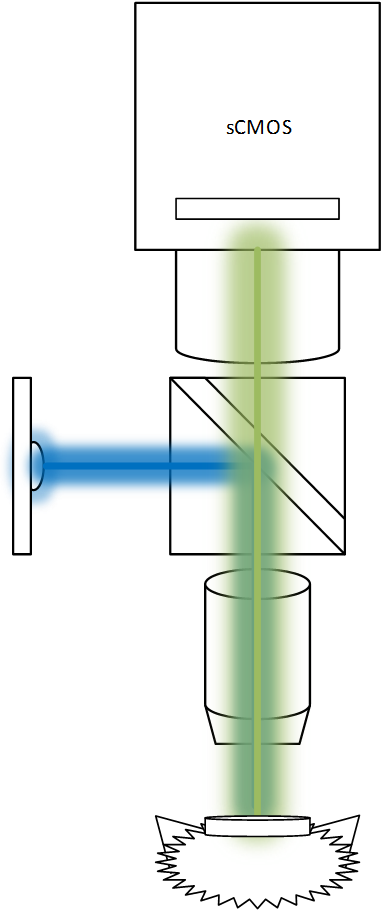
\includegraphics[height=8cm]{2_body/figures/widefield_microscope_diagram.png} \medskip \centerline{(a)}
	\end{minipage}
	\hfill
	\begin{minipage}[t]{0.49\linewidth}\centering 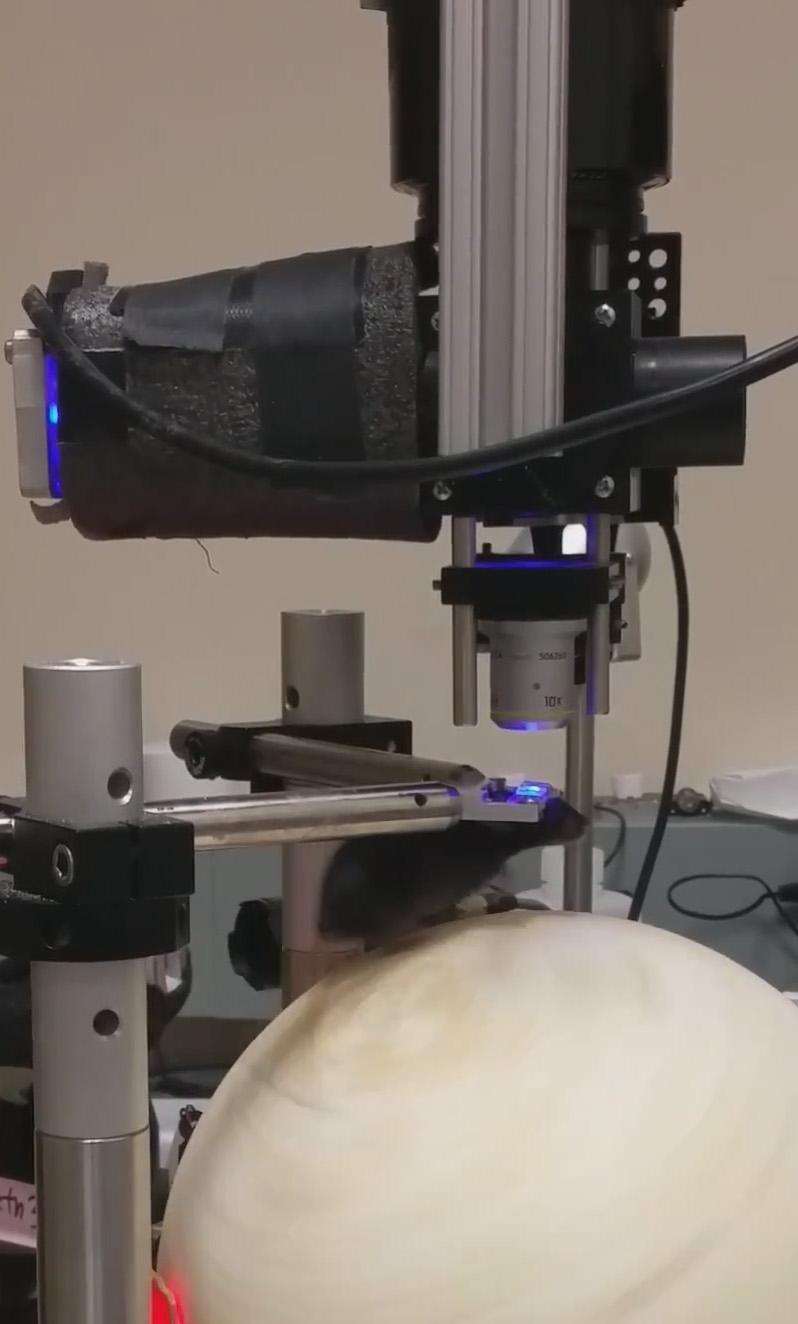
\includegraphics[height=8cm]{2_body/figures/setup1.jpg} \medskip \centerline{(b)}
	\end{minipage}
	\caption{Basic configuration for a widefield epifluorescence microscope for in-vivo imaging.
		This first configuration used a phase contrast lens borrowed from an inverted microscope (not recommended).
		(a) Schematic showing relation of microscope and mouse on spherical treadmill; (b) Setup 1: the LED used for extending to the left (black covering to block light)}
	\label{fig:Sampling}
\end{figure}

\begin{figure}[htb]
	\begin{minipage}[t]{0.45\linewidth}\centering
		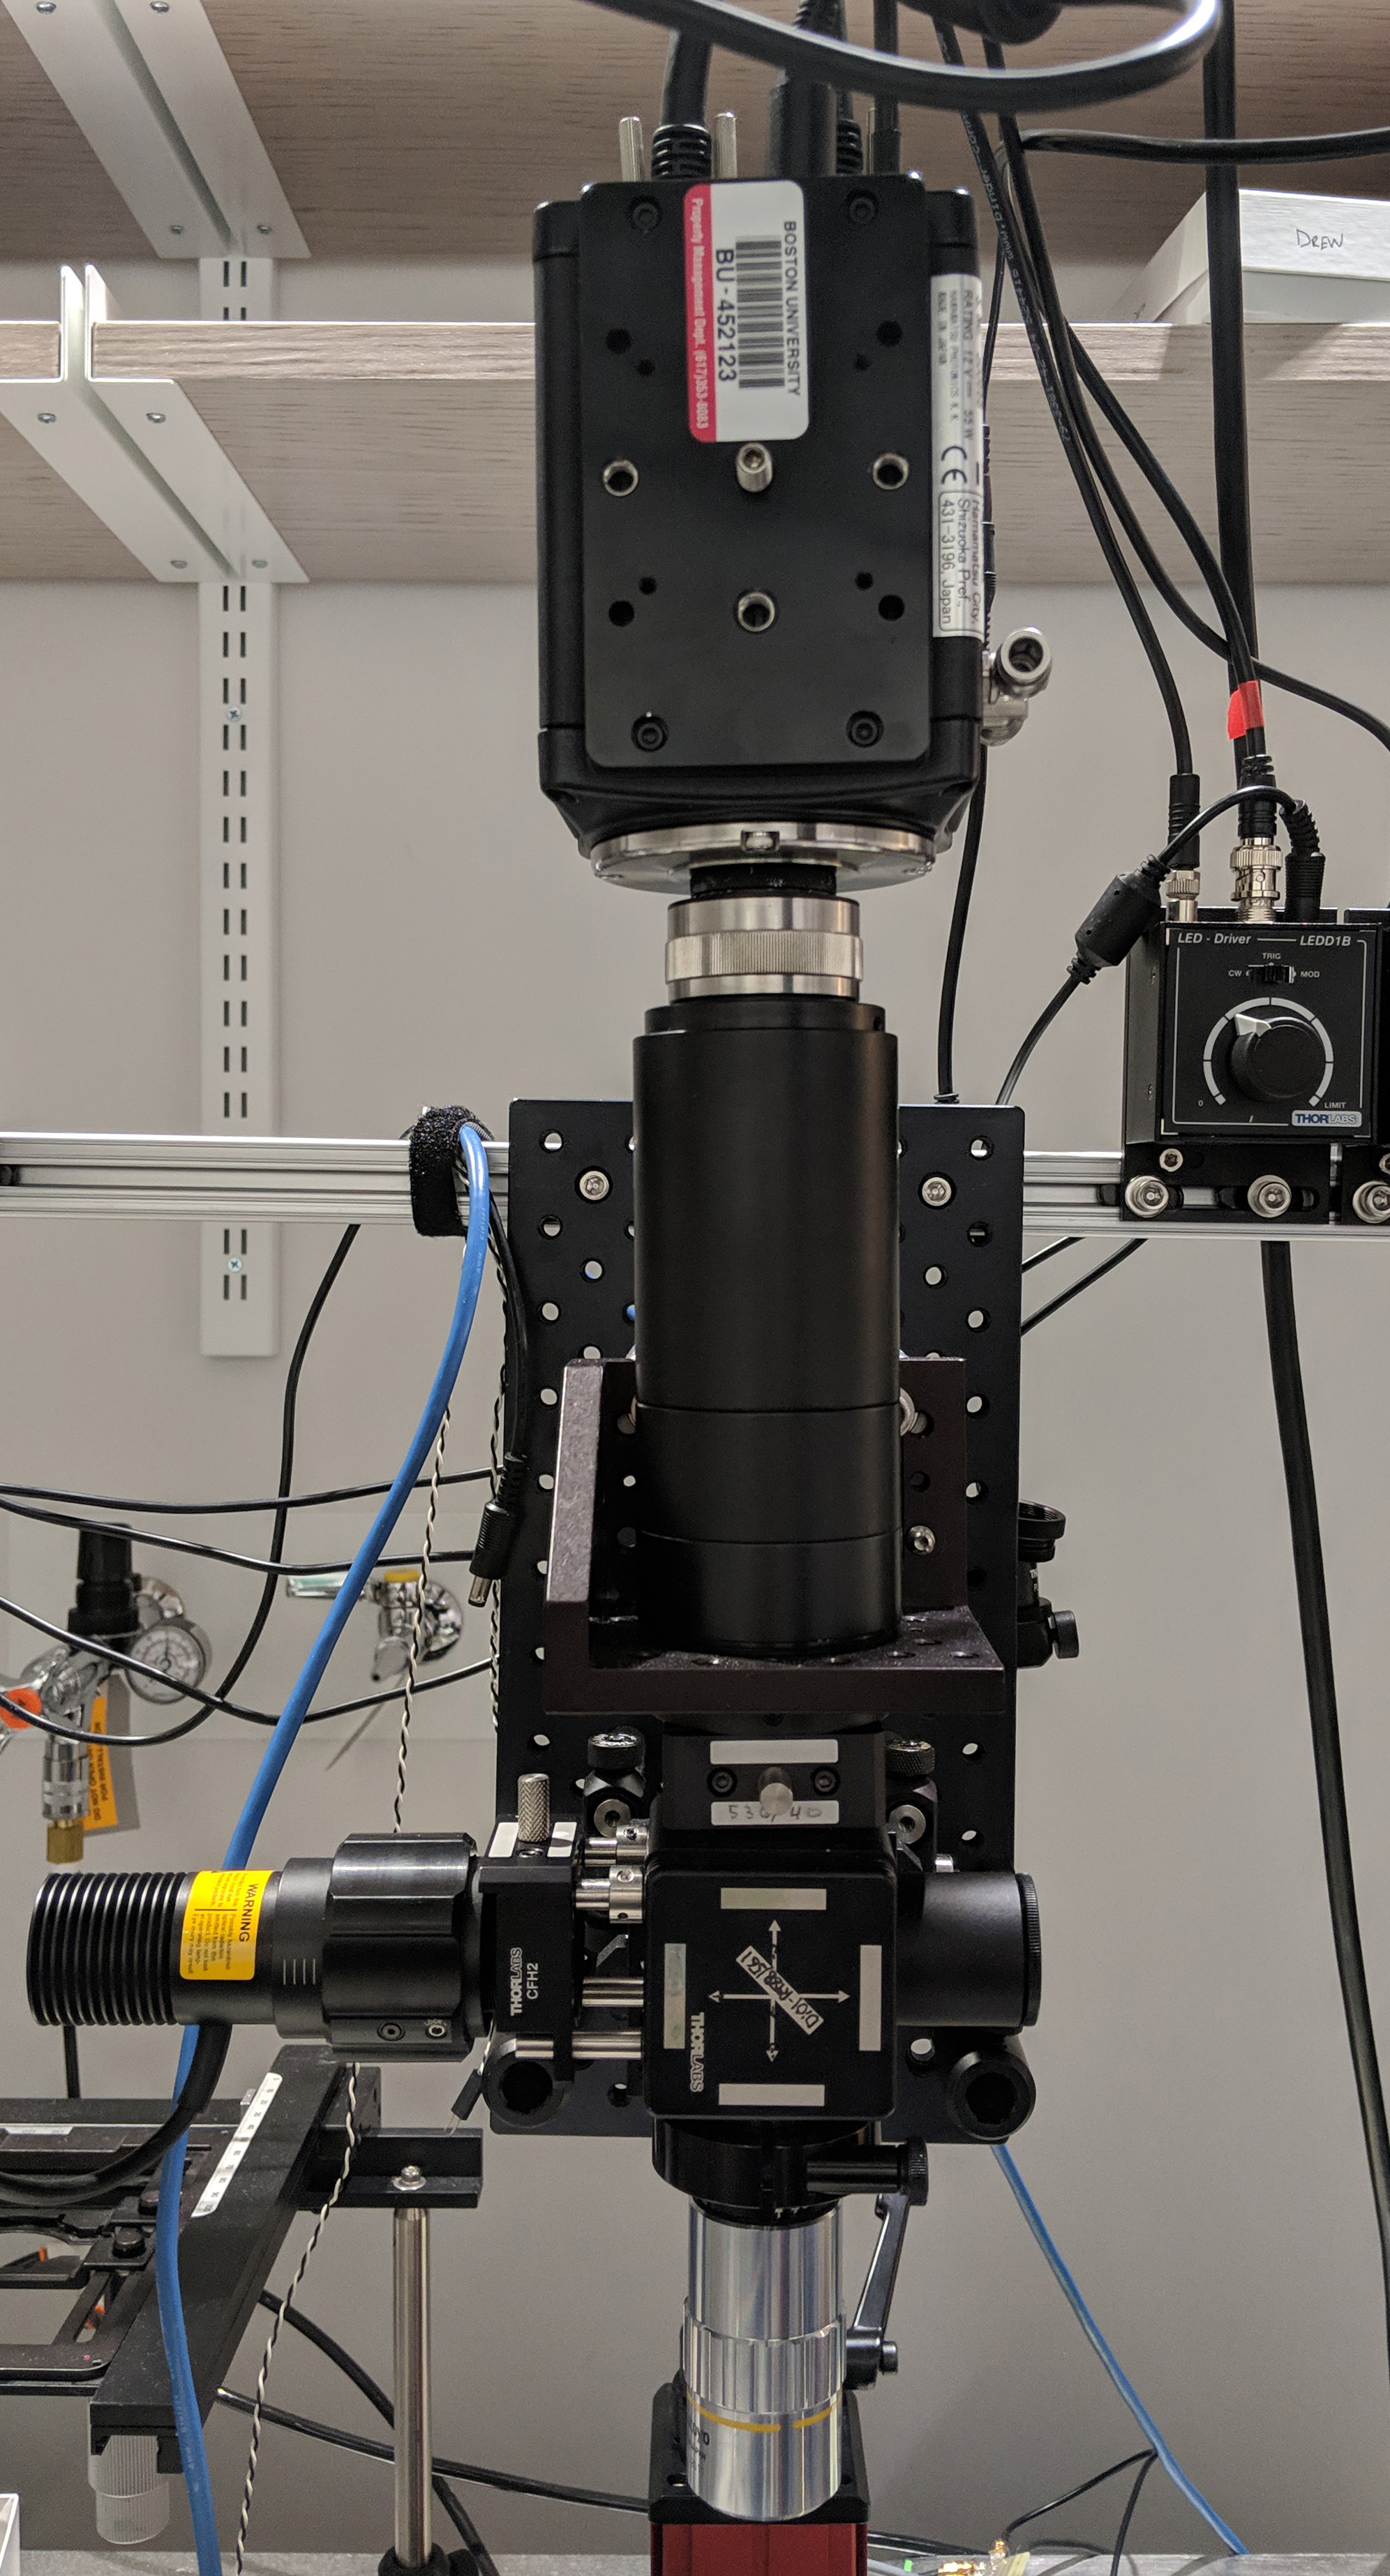
\includegraphics[height=10cm]{2_body/figures/setup3-front.jpg}
		\centerline{(a)}
	\end{minipage}
	\hfill
	\begin{minipage}[t]{0.45\linewidth}\centering
		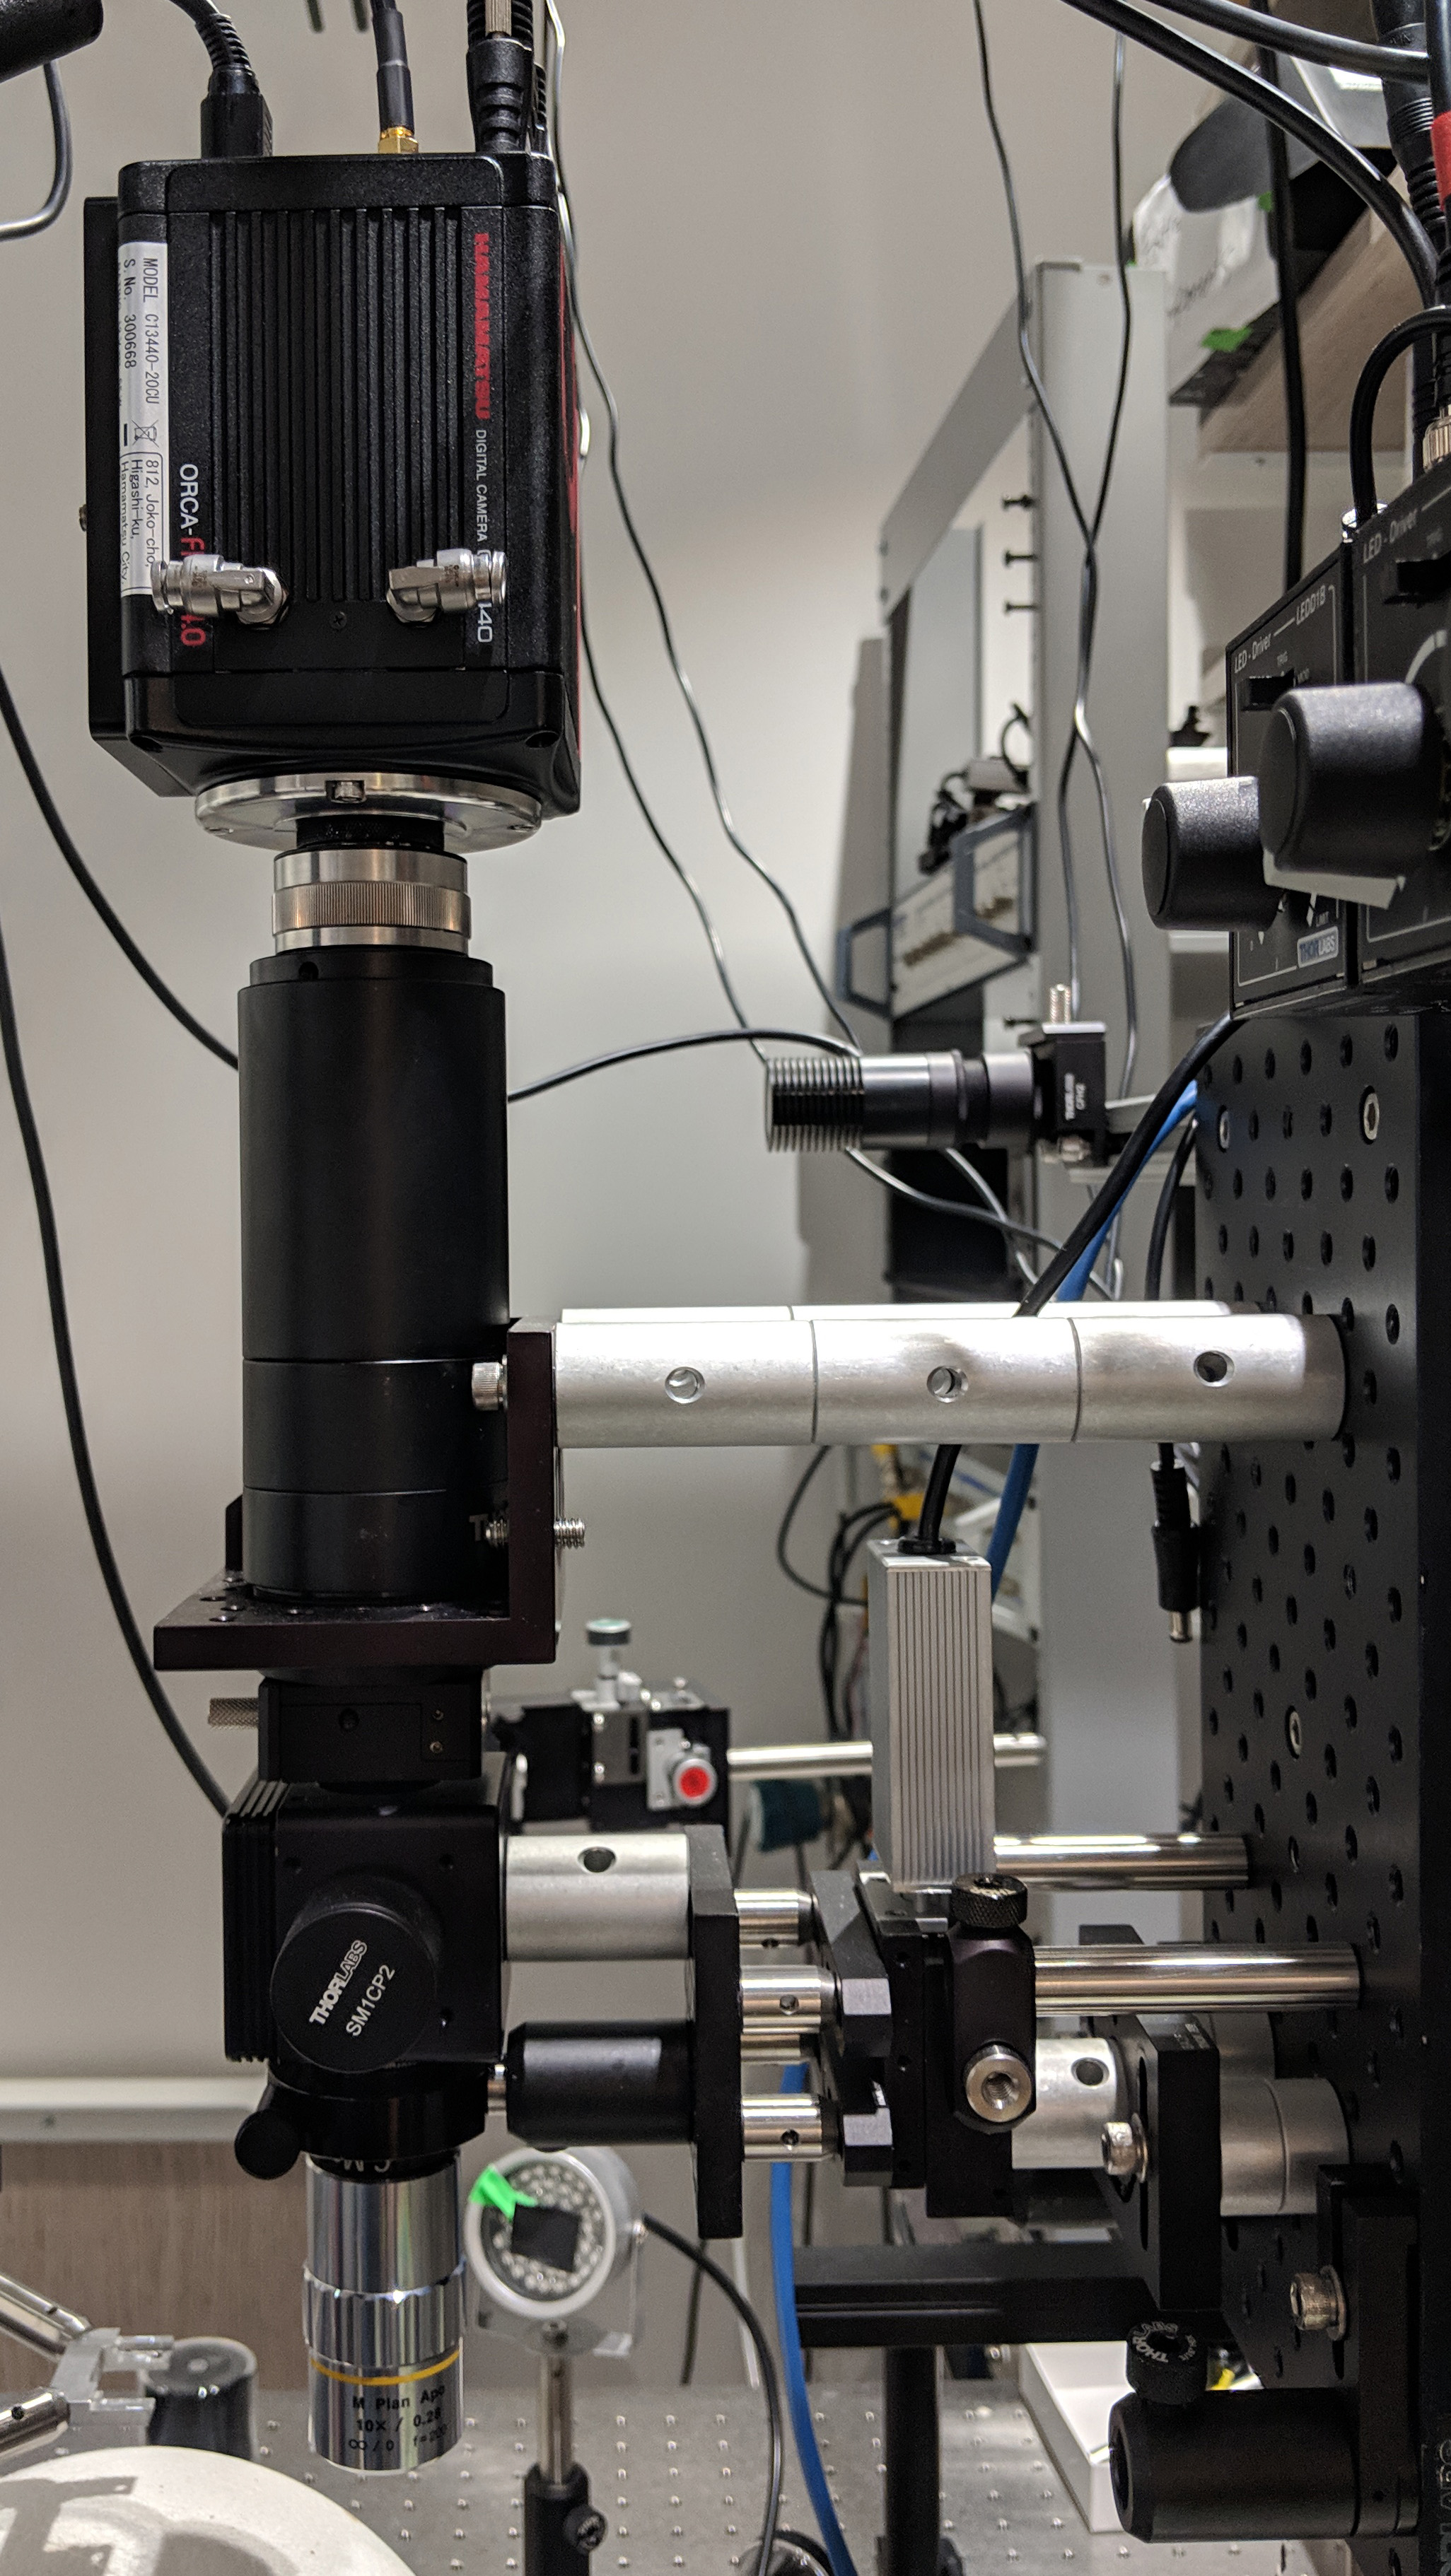
\includegraphics[height=10cm]{2_body/figures/setup3-side.jpg}
		\centerline{(b)}
	\end{minipage}
	\begin{minipage}[t]{\linewidth}\centering
		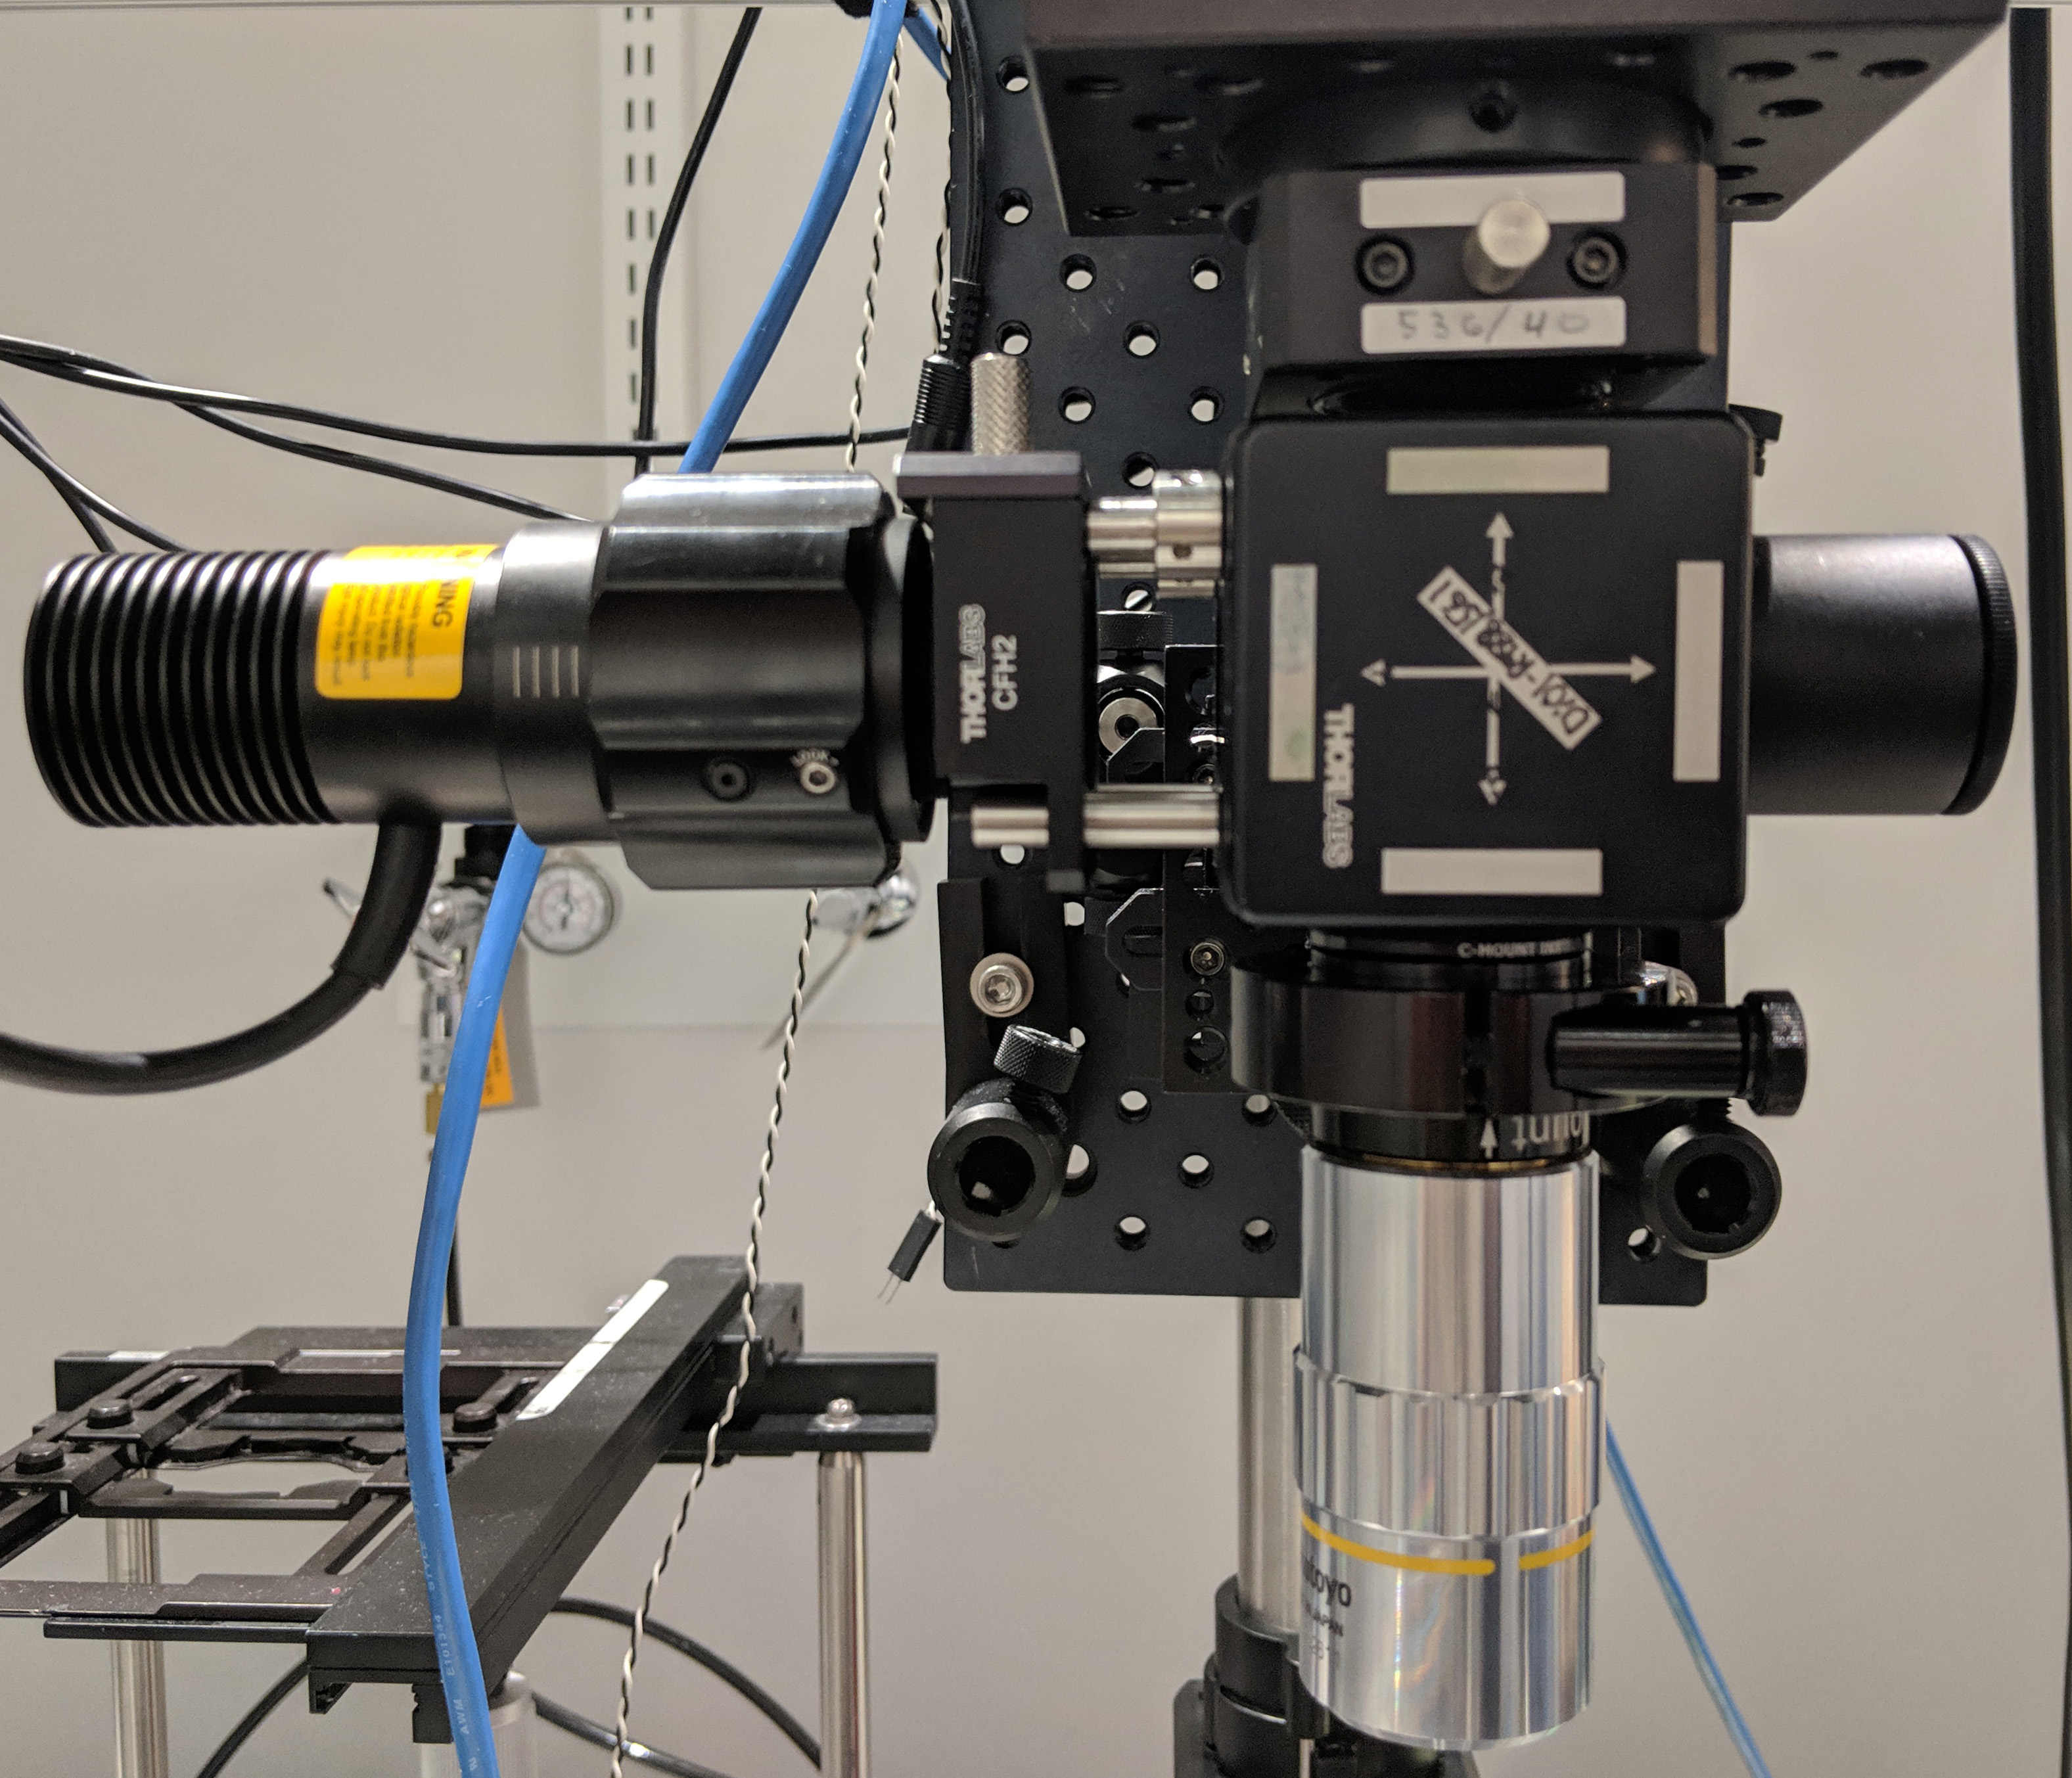
\includegraphics[width=7cm]{2_body/figures/setup3-closeup.jpg}
		\centerline{(c)}
	\end{minipage}
	\caption{
		Microscope Setup 2 (a) front;
		(b) close up; (c) side}
	\label{fig:motion sensors}
\end{figure}

\begin{figure}[htb]
	\begin{minipage}[t]{0.32\linewidth}\centering
		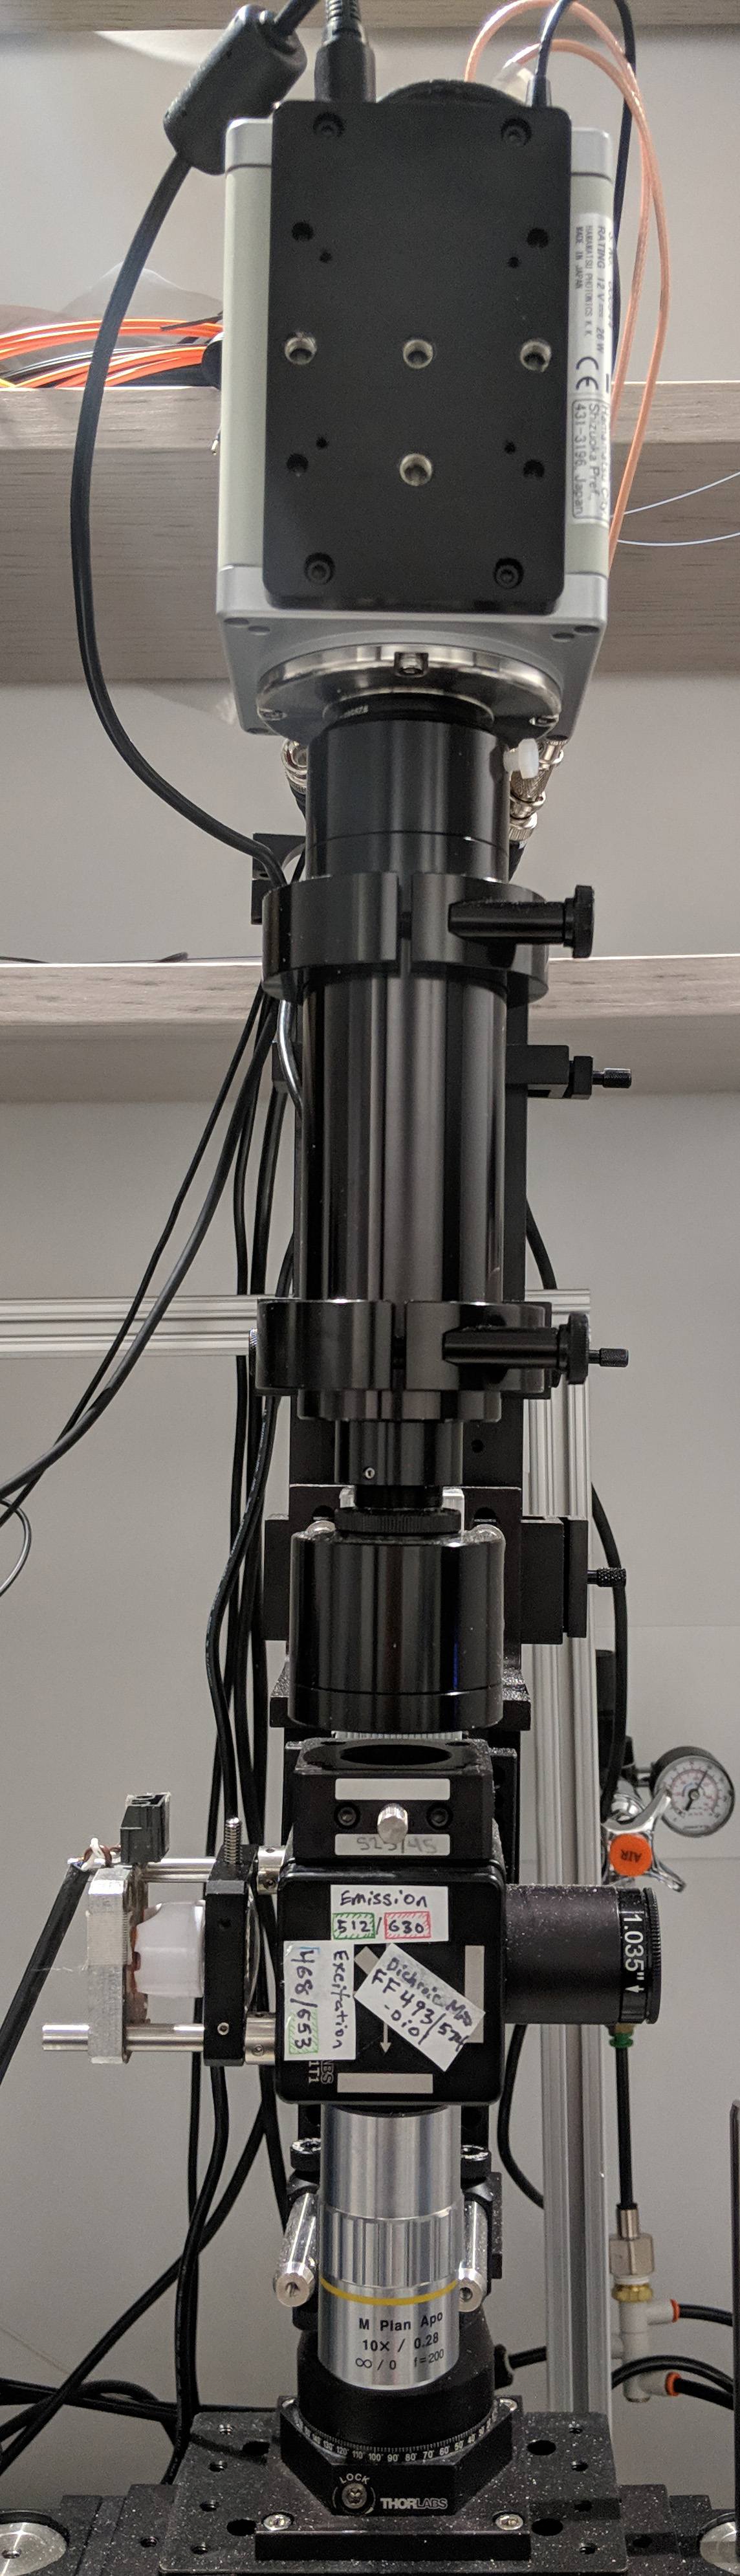
\includegraphics[width=4cm]{2_body/figures/setup4-front.jpg}
		\centerline{(a)}
	\end{minipage}
	\hfill
	\begin{minipage}[t]{0.32\linewidth}\centering
		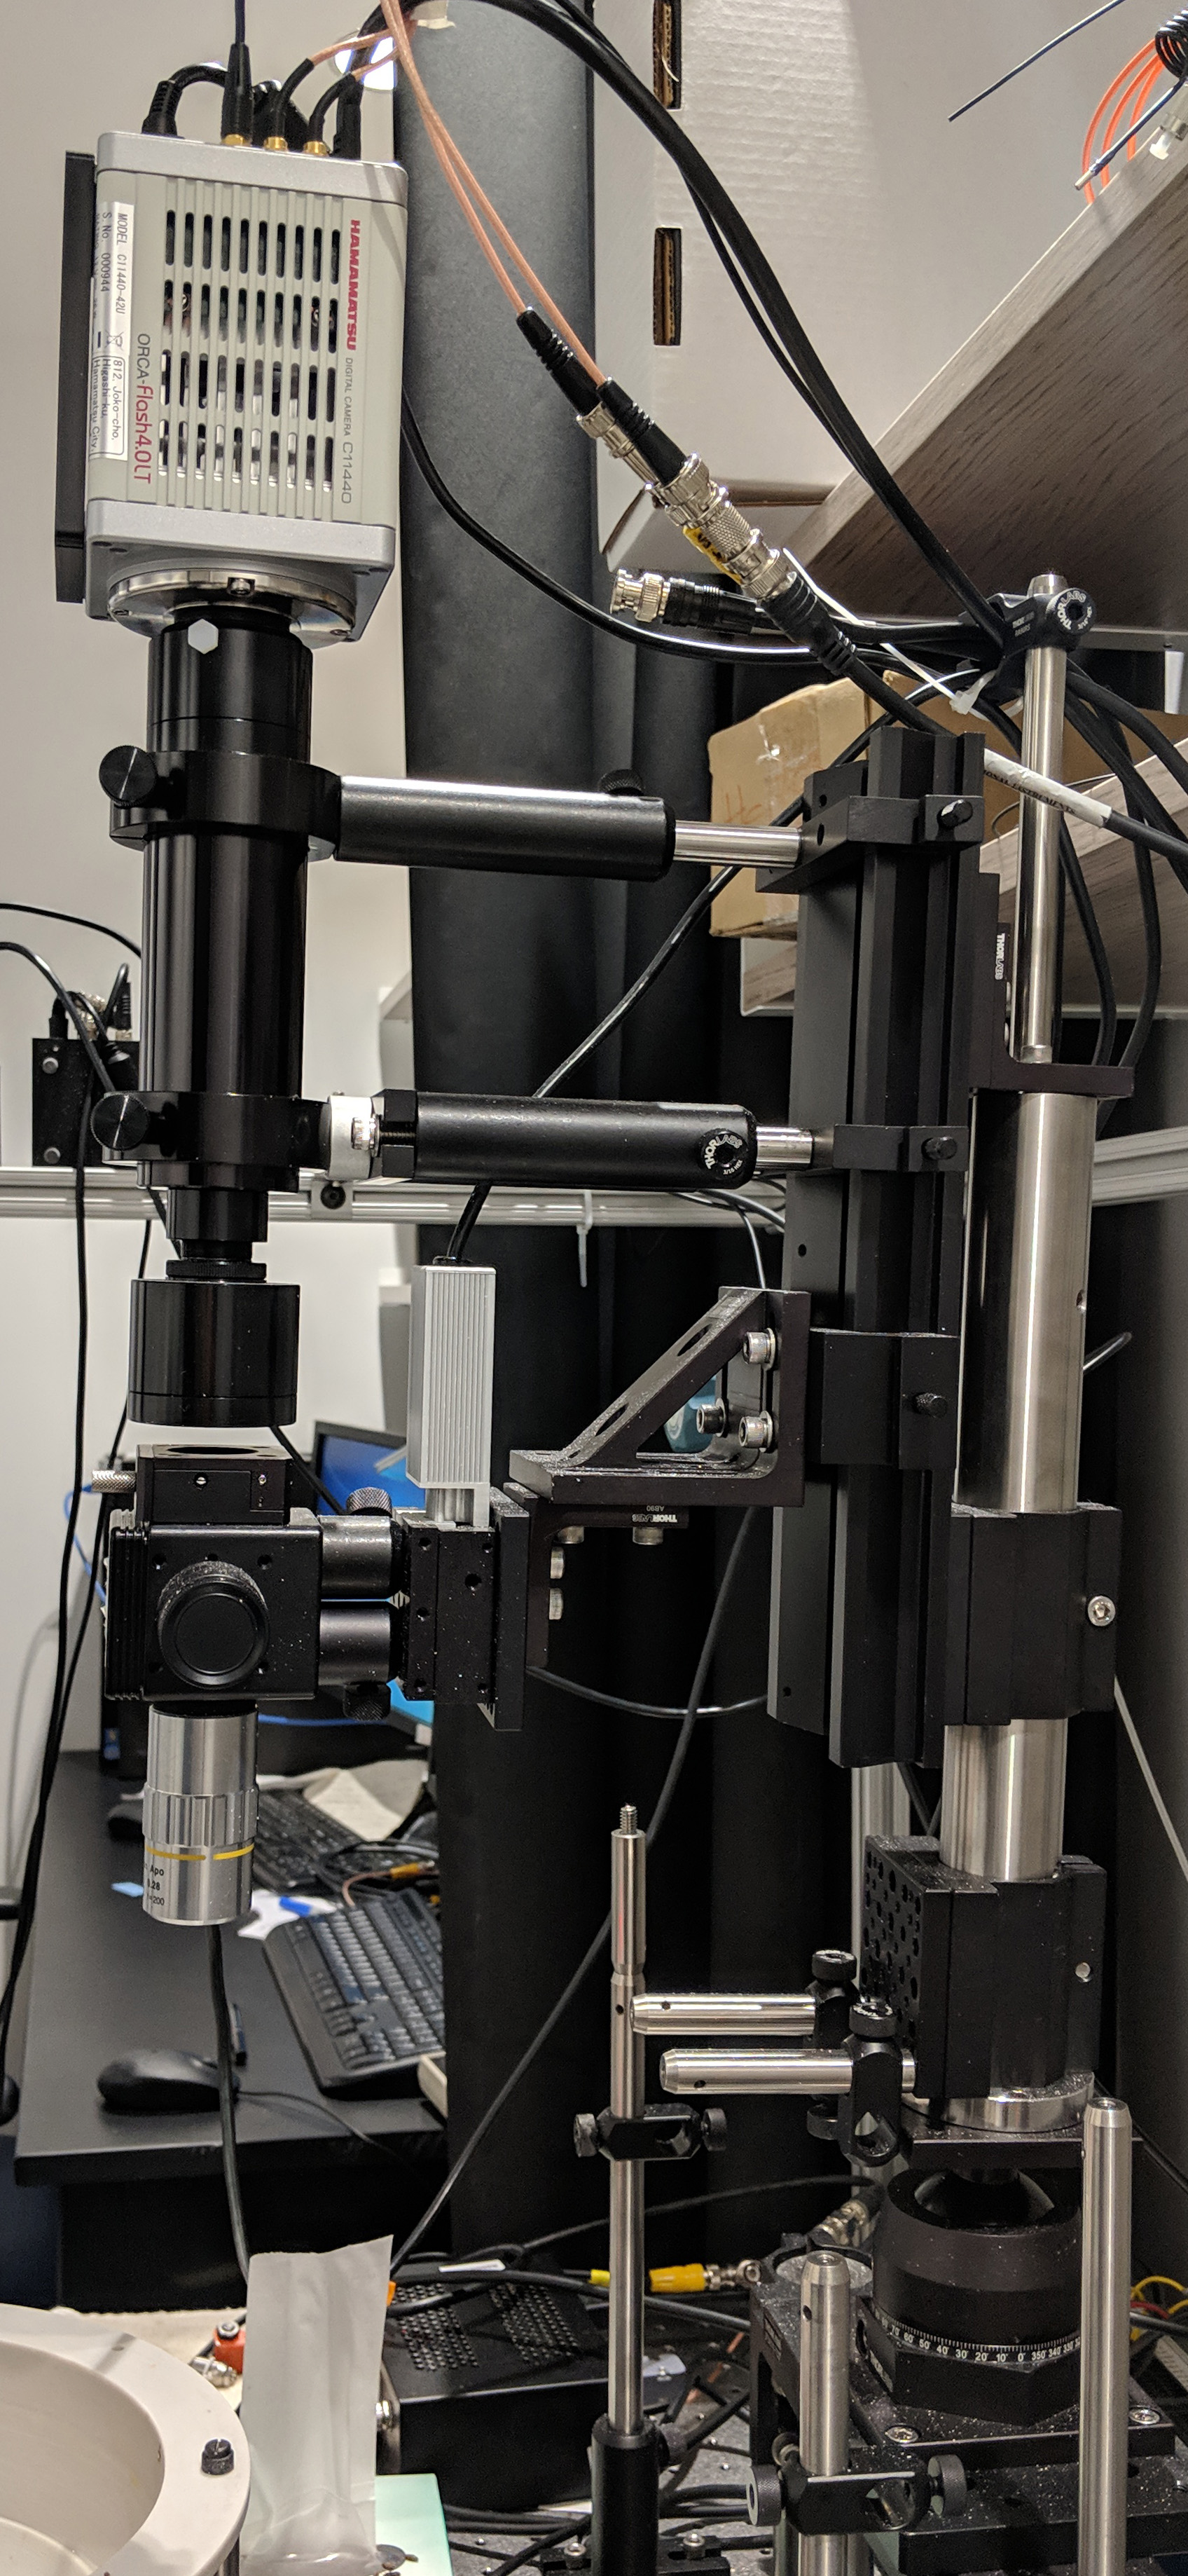
\includegraphics[width=4cm]{2_body/figures/setup4-side.jpg}
		\centerline{(b)}
	\end{minipage}
	\begin{minipage}[t]{0.32\linewidth}\centering
		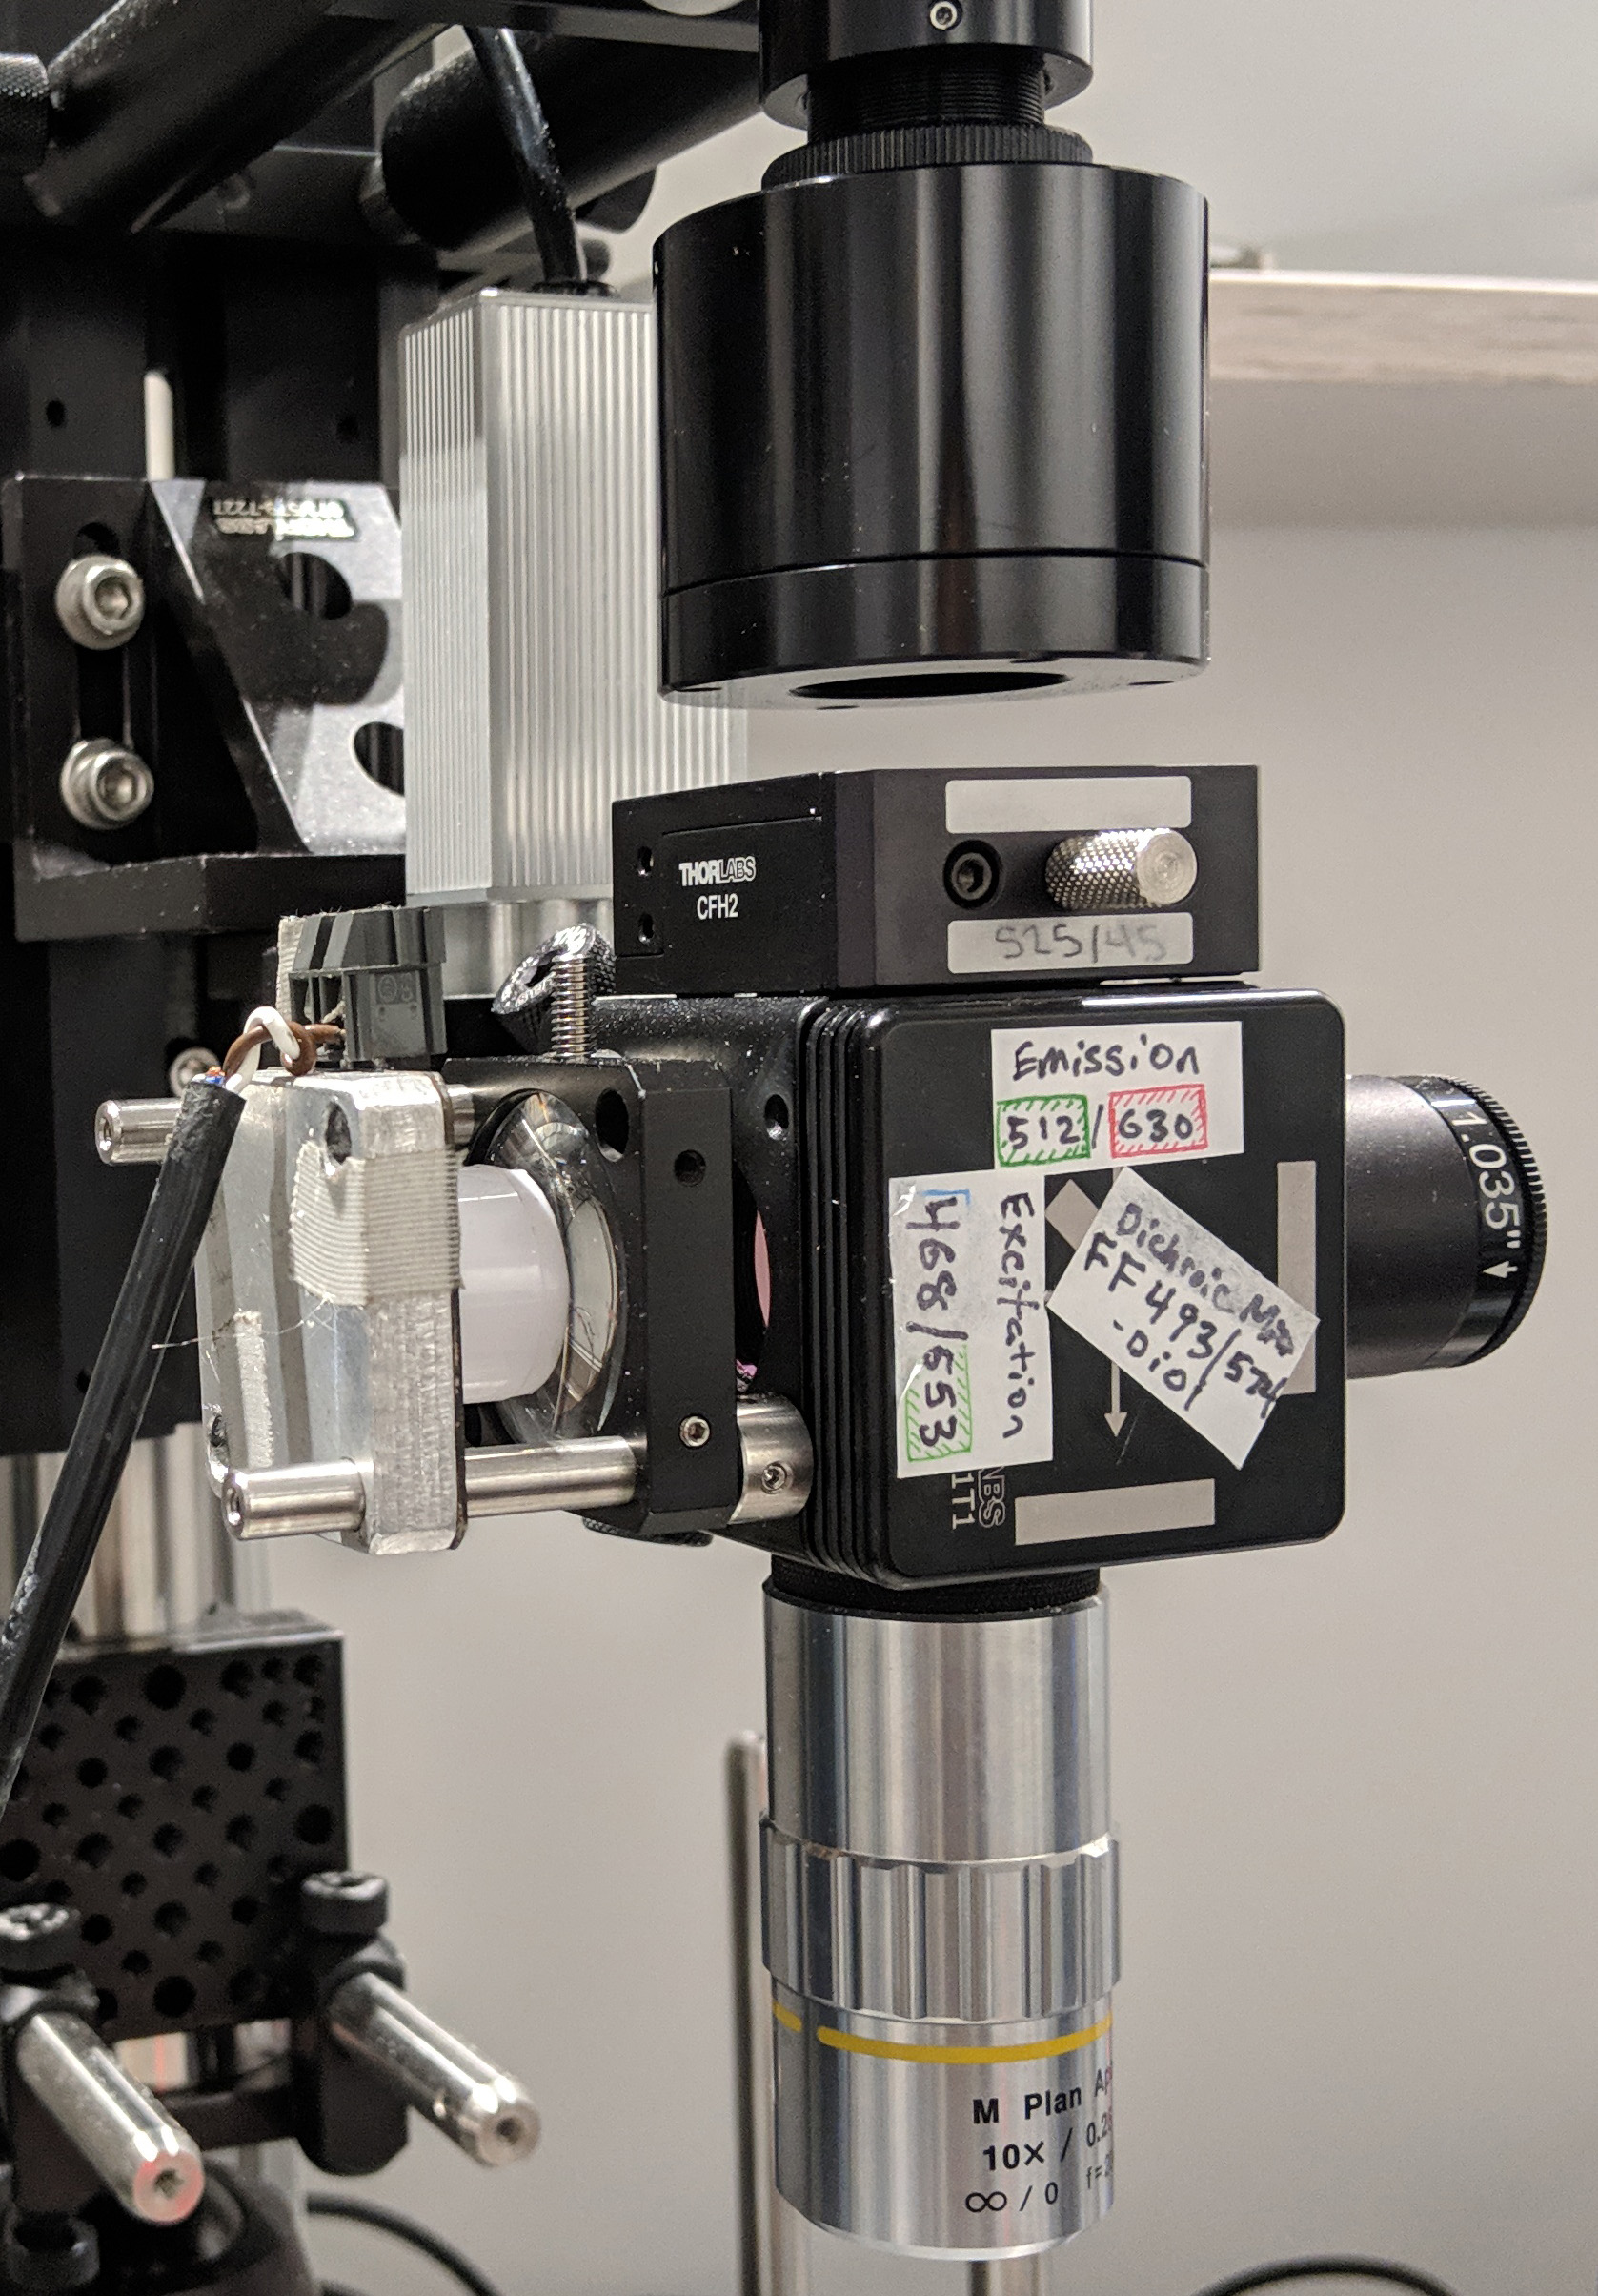
\includegraphics[width=4cm]{2_body/figures/setup4-closeup.jpg}
		\centerline{(c)}
	\end{minipage}
	\caption{
		Widefield fluorescence microscope reconfigured Setup 3.
		Multiple iterations are shown, with later iterations offering improved compatibility with usage of off-the-shelf components.
		(a) front; (b) close up; (c) side}
	\label{fig:motion sensors}
\end{figure}

%You will also be using a lot of citations. Here is the format required in the dissertation: \cite{lamport1985:latex},\cite{Debr01}.

\clearpage

\end{document}
